\documentclass[hyperref={bookmarks=false},aspectratio=169]{beamer}
\usepackage{hyperref,ragged2e,amsmath,amssymb,url,bm}
\usepackage{graphicx,booktabs,array}
\usepackage{tikz}
\usetikzlibrary{arrows.meta,positioning,calc,shapes.geometric,decorations.pathreplacing,matrix}
\graphicspath{{crops/}}
\usetheme{Goettingen}
% --- Paleta: azul profundo, dorado y papiro crema ---
\definecolor{azul}{HTML}{15437C}
\definecolor{azuloscuro}{HTML}{0B1F3A}
\definecolor{celeste}{HTML}{5694D6}
\definecolor{dorado}{RGB}{196,154,60}
\definecolor{papiro}{RGB}{246,239,220}
\definecolor{gris}{RGB}{70,78,96}
\setbeamercolor{structure}{fg=azul}
\setbeamertemplate{sidebar canvas right}[vertical shading][top=azul,bottom=azuloscuro]
\setbeamercolor{title in sidebar}{fg=dorado}
\setbeamercolor{author in sidebar}{fg=papiro}
\setbeamercolor{section in sidebar}{fg=papiro}
\setbeamercolor{section in sidebar shaded}{fg=dorado!70!papiro}
\setbeamercolor{subsection in sidebar}{fg=papiro}
\setbeamercolor{subsection in sidebar shaded}{fg=dorado!70!papiro}
\let\raggedright\justifying
\setlength{\RaggedRightRightskip}{0pt plus 1fil}
\setbeamertemplate{background canvas}{
\includegraphics[width=\paperwidth,height=\paperheight]{papiro.jpg}}
\setbeamercolor{normal text}{fg=black!88!azuloscuro}
\setbeamercolor{frametitle}{fg=azul}
\setbeamerfont{frametitle}{series=\bfseries}
\setbeamertemplate{section in toc shaded}{\leavevmode{\color{gris}\inserttocsection}\par}
\setbeamercolor{title}{fg=azul}
\setbeamercolor{subtitle}{fg=gris}
\setbeamercolor{item projected}{bg=azul,fg=papiro}
\setbeamertemplate{itemize item}{\small\textcolor{dorado}{$\blacktriangleright$}}
\setbeamertemplate{navigation symbols}{}
% --- Español + hebreo + griego (XeLaTeX) ---
\usepackage[bidi=default]{babel}
\babelprovide[import,main]{spanish}
\babelprovide[import]{hebrew}
\babelprovide[import]{ancientgreek}
\babelfont[hebrew]{sf}[Path=fonts/, BoldFont=NotoHebrewSans-700.ttf]{NotoHebrewSans-400.ttf}
\babelfont[hebrew]{rm}[Path=fonts/, BoldFont=NotoHebrewSans-700.ttf]{NotoHebrewSans-400.ttf}
\babelfont[ancientgreek]{sf}[Path=fonts/]{GFSPorson.otf}
\babelfont[ancientgreek]{rm}[Path=fonts/]{GFSPorson.otf}
\newcommand{\heb}[1]{\mbox{\foreignlanguage{hebrew}{#1}}}
\newcommand{\grc}[1]{\foreignlanguage{ancientgreek}{#1}}
\newcommand{\SENOR}{S{\fontsize{0.78em}{1em}\selectfont EÑOR}}
% --- Citas (cuadro de un solo color), imágenes, referencias ---
\usepackage[most]{tcolorbox}
\newtcolorbox{cita}[1][]{enhanced, colback=azul!7!papiro, opacityback=0.85, colframe=azul,
  boxrule=0pt, leftrule=2.5pt, arc=0pt, left=6pt, right=6pt, top=4pt, bottom=4pt,
  before skip=4pt, after skip=6pt, fontupper=\small\itshape, #1}
\newcommand{\fuente}[1]{\par\hfill{\upshape\bfseries\footnotesize\textcolor{azul}{#1}}}
\makeatletter
\newcommand{\fotolado}[2]{%
  \begin{tikzpicture}[remember picture,overlay]
    \node[anchor=north east,inner sep=0pt] (foto) at ([xshift=-\beamer@sidebarwidth]current page.north east)
      {\includegraphics[height=\paperheight]{#1}};
    \node[anchor=south east,inner sep=2pt,text=papiro,fill=azuloscuro,fill opacity=0.6,text opacity=1,
      font=\fontsize{4.5}{5.5}\selectfont,align=right,text width=4.2cm] at ([xshift=-3pt,yshift=3pt]foto.south east)
      {\textit{Nota.} #2};
  \end{tikzpicture}}
\makeatother
\newcommand{\refapa}[1]{\par{\RaggedRight\hangindent=1.2em\hangafter=1\noindent #1\par}\vspace{3pt}}
\usepackage{xurl}\urlstyle{same}
\newcommand{\destacar}[1]{\textbf{\textcolor{azul}{#1}}}
\newcommand{\precision}[1]{{\footnotesize\color{gris}\textbf{Precisión:} #1}}
\tikzset{caja/.style={draw=azul,line width=0.8pt,fill=papiro,fill opacity=0.92,text opacity=1,rounded corners=3pt,inner sep=5pt,font=\scriptsize}}
\title[Dios es Espíritu]{\bfseries{Dios es Espíritu}}
\subtitle{``Dios es Espíritu; y los que le adoran, en espíritu y en verdad es necesario que adoren'' (Jn 4:24)}
\author{}\institute{}\date{}
\titlegraphic{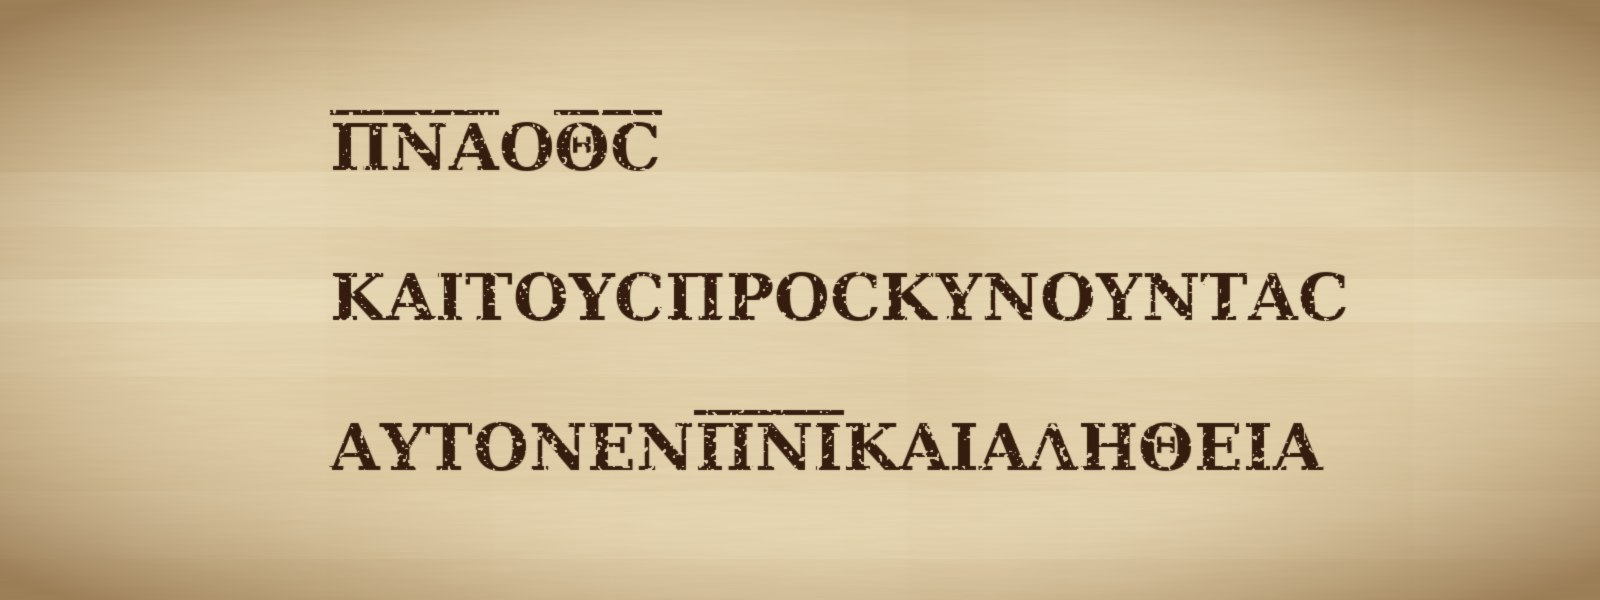
\includegraphics[width=0.80\linewidth,height=0.36\textheight,keepaspectratio]{portada.jpg}\\[-1pt]
  {\fontsize{5}{6}\selectfont\color{gris}\textit{Nota.} Elaboración propia: Jn 4:24 en escritura uncial (texto NA28), con \emph{nomina sacra}.}}
\AtBeginSection[]{\begin{frame}\frametitle{Contenidos}\tableofcontents[currentsection]\end{frame}}
\begin{document}
\frame{\titlepage}

\begin{frame}\frametitle{Contenidos}\tableofcontents\end{frame}

% ------------------------------------------------------------------
\section{Contexto}

\begin{frame}{Tres palabras en un pozo}
\begin{columns}[c,onlytextwidth]
\begin{column}{0.50\textwidth}
\begin{cita}Dios es Espíritu; y los que le adoran, en espíritu y en verdad es necesario que adoren.\fuente{(Jn 4:24, RVR1960)}\end{cita}
\begin{center}\grc{πνεῦμα ὁ θεός}\end{center}
\scriptsize Tres palabras griegas: ``espíritu (es) Dios''. La definición más breve de Dios en la Biblia se dijo a una mujer samaritana, junto a un pozo, a mediodía.
\end{column}
\begin{column}{0.48\textwidth}\small
\begin{itemize}
\item La mujer pregunta por un \destacar{lugar}: ¿Gerizim o Jerusalén?
\item Jesús responde con el \destacar{ser} de Dios: porque Dios es Espíritu, el lugar deja de ser la pregunta.
\item El atributo no se presenta como especulación: se presenta como la razón de una \destacar{adoración} nueva.
\end{itemize}
\end{column}
\end{columns}
\end{frame}

\begin{frame}{Un atributo del Ser}
\begin{columns}[c,onlytextwidth]
\begin{column}{0.50\textwidth}
\centering
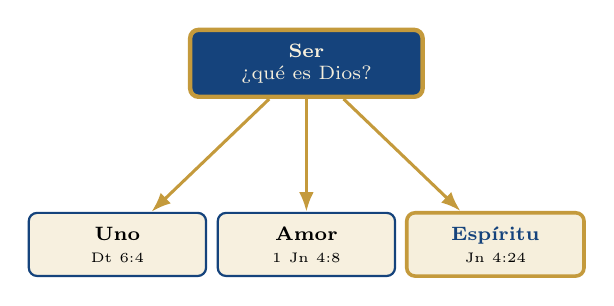
\begin{tikzpicture}[font=\scriptsize]
 \node[draw=dorado,line width=1.6pt,fill=azul,text=papiro,rounded corners=3pt,text width=2.6cm,align=center,inner sep=5pt] (s) at (0,1.9) {\textbf{Ser}\\ ¿qué es Dios?};
 \node[caja,text width=1.9cm,align=center] (u) at (-2.4,-0.4) {\textbf{Uno}\\ {\tiny Dt 6:4}};
 \node[caja,text width=1.9cm,align=center] (a) at (0,-0.4) {\textbf{Amor}\\ {\tiny 1 Jn 4:8}};
 \node[draw=dorado,line width=1.3pt,fill=papiro,rounded corners=3pt,text width=1.9cm,align=center,inner sep=5pt] (e) at (2.4,-0.4) {\textbf{\textcolor{azul}{Espíritu}}\\ {\tiny Jn 4:24}};
 \foreach \i in {u,a,e}\draw[-{Latex[length=2.5mm]},dorado,line width=1.1pt](s)--(\i);
\end{tikzpicture}
\end{column}
\begin{column}{0.48\textwidth}\small
\begin{itemize}
\item La serie agrupa en el \destacar{Ser} lo que responde a ``¿qué es Dios?'': Uno, Amor, Espíritu.
\item Juan da tres fórmulas con ``Dios es'': \emph{Espíritu} (Jn 4:24), \emph{luz} (1 Jn 1:5), \emph{amor} (1 Jn 4:8).
\item Pink las reúne como ``tres cosas'' que la Escritura dice de la naturaleza de Dios (Pink, 2020, cap. 16).
\end{itemize}
\end{column}
\end{columns}\par\smallskip
\precision{clasificación propuesta: atributo del Ser; \emph{incomunicable} en su esencia (Dios es espíritu increado, infinito y fuente de todo espíritu), \emph{comunicable} como reflejo (Dios ``forma el espíritu del hombre dentro de él'', Zac 12:1).}
\end{frame}

\begin{frame}{``Espíritu'' en la Biblia}
\begin{columns}[c,onlytextwidth]
\begin{column}{0.40\textwidth}\footnotesize
\begin{itemize}
\item RVR1960: ``espíritu, espíritus, espiritual(es), espiritualmente'' \textbf{674 veces} en \textbf{607 versículos} (262 AT, 412 NT).
\item Hebreo: \heb{רוּחַ} \emph{rúaj} ``se encuentra unas 378 veces'' (Vine).
\item Griego NT: \grc{πνεῦμα} \emph{pneûma}, \textbf{379 veces} en 344 versículos.
\item La misma palabra dice \destacar{viento}, \destacar{aliento} y \destacar{espíritu}.
\end{itemize}
\end{column}
\begin{column}{0.58\textwidth}
\scriptsize\renewcommand{\arraystretch}{1.12}
\begin{tabular}{@{}>{\RaggedRight\arraybackslash}p{3.6cm}>{\RaggedRight\arraybackslash}p{2.4cm}r@{}}
\toprule
\textbf{Forma (RVR1960)} & \textbf{Original más frecuente} & \textbf{Veces} \\ \midrule
espíritu & \heb{רוּחַ}, \grc{πνεῦμα} & 608 \\
espíritus & \heb{רוּחוֹת}, \grc{πνεύματα} & 36 \\
espiritual & \grc{πνευματικός} & 19 \\
espirituales & \grc{πνευματικός} & 10 \\
espiritualmente & \grc{πνευματικῶς} & 1 \\ \midrule
\textbf{Total} & & \textbf{674} \\
\bottomrule
\end{tabular}
\end{column}
\end{columns}\par\smallskip
\precision{conteo propio con la RVR1960 sin títulos de sección y con números Strong; NA27 para el griego. Verificar en e-Sword.}
\end{frame}

% ------------------------------------------------------------------
\section{Juan 4}

\begin{frame}{Sicar, el pozo de Jacob}
\centering
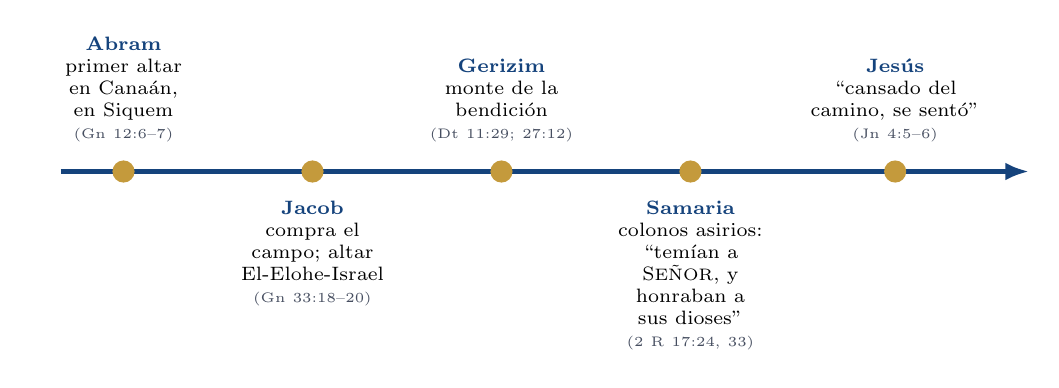
\begin{tikzpicture}[font=\scriptsize]
 \draw[line width=1.6pt,azul,-{Latex[length=3mm]}] (-0.3,0) -- (12.0,0);
 \foreach \x/\t/\b/\r/\pos in {0.5/{Abram}/{primer altar en Canaán, en Siquem}/{Gn 12:6--7}/above,
   2.9/{Jacob}/{compra el campo; altar El-Elohe-Israel}/{Gn 33:18--20}/below,
   5.3/{Gerizim}/{monte de la bendición}/{Dt 11:29; 27:12}/above,
   7.7/{Samaria}/{colonos asirios: ``temían a \SENOR, y honraban a sus dioses''}/{2 R 17:24, 33}/below,
   10.3/{Jesús}/{``cansado del camino, se sentó''}/{Jn 4:5--6}/above}{
  \fill[dorado] (\x,0) circle (4pt);
  \node[\pos=7pt,text width=2.2cm,align=center] at (\x,0) {\textbf{\textcolor{azul}{\t}}\\ \b\\ {\tiny\color{gris}(\r)}};}
\end{tikzpicture}\par\medskip
\begin{columns}[t,onlytextwidth]
\begin{column}{0.49\textwidth}
\begin{cita}Vino, pues, a una ciudad de Samaria llamada Sicar, junto a la heredad que Jacob dio a su hijo José. Y estaba allí el pozo de Jacob.\fuente{(Jn 4:5--6, RVR1960)}\end{cita}
\end{column}
\begin{column}{0.49\textwidth}\small
El diálogo ocurre en tierra de patriarcas: Siquem, Jacob, José. La mujer lo sabe: ``Nuestros padres adoraron en este monte'' (4:20). La pregunta del lugar tiene siglos de historia.
\end{column}
\end{columns}
\end{frame}

\begin{frame}{¿Este monte o Jerusalén?}
\scriptsize\renewcommand{\arraystretch}{1.18}
\begin{tabular}{@{}>{\RaggedRight\arraybackslash}p{2.6cm}>{\RaggedRight\arraybackslash}p{4.6cm}>{\RaggedRight\arraybackslash}p{4.6cm}@{}}
\toprule
 & \textbf{Samaritanos: Gerizim} & \textbf{Judíos: Jerusalén} \\ \midrule
Canon & solo el Pentateuco & Ley, Profetas y Escritos \\
Base & altares de Abram y Jacob en Siquem (Gn 12:6--7; 33:20); la bendición en Gerizim (Dt 11:29; 27:12) & ``el lugar que \SENOR{} vuestro Dios escogiere'' (Dt 12:5), identificado con Sion (2 Cr 6:6; Sal 132:13) \\
Texto & el Pentateuco samaritano lee ``Gerizim'' en Dt 27:4 (TM: ``Ebal'') y añade Gerizim al Decálogo & el TM lee ``Ebal'' en Dt 27:4 \\
Templo & construido en Gerizim; destruido por Juan Hircano (129 a.\,e.\,c.) & segundo templo, en pie en tiempos de Jesús \\
\bottomrule
\end{tabular}\par\medskip
\begin{columns}[t,onlytextwidth]
\begin{column}{0.52\textwidth}
\begin{cita}Nuestros padres adoraron en este monte, y vosotros decís que en Jerusalén es el lugar donde se debe adorar.\fuente{(Jn 4:20, RVR1960)}\end{cita}
\end{column}
\begin{column}{0.46\textwidth}
\precision{(textual) lecturas del Pentateuco samaritano según Tov (2012) y la \emph{Encyclopaedia Judaica} (2007, ``Gerizim, Mount''), que fecha la destrucción del templo en 129 a.\,e.\,c. (Josefo, \emph{Ant.} 13.255--256). Base samaritana resumida según MacArthur (notas a Jn 4:20).}
\end{column}
\end{columns}
\end{frame}

\begin{frame}{Texto ancla: Jn 4:19--24}
\fotolado{panel_juan4.jpg}{Elaboración propia: Jn 4:24 en escritura uncial (texto NA28), con \emph{nomina sacra}.}
\begin{columns}[c,onlytextwidth]
\begin{column}{0.58\textwidth}
\begin{cita}[fontupper=\scriptsize\itshape]Le dijo la mujer: Señor, me parece que tú eres profeta. Nuestros padres adoraron en este monte, y vosotros decís que en Jerusalén es el lugar donde se debe adorar. Jesús le dijo: Mujer, créeme, que la hora viene cuando ni en este monte ni en Jerusalén adoraréis al Padre. Vosotros adoráis lo que no sabéis; nosotros adoramos lo que sabemos; porque la salvación viene de los judíos. Mas la hora viene, y ahora es, cuando los verdaderos adoradores adorarán al Padre en espíritu y en verdad; porque también el Padre tales adoradores busca que le adoren. Dios es Espíritu; y los que le adoran, en espíritu y en verdad es necesario que adoren.\fuente{(Jn 4:19--24, RVR1960)}\end{cita}
\end{column}
\begin{column}{0.40\textwidth}\end{column}
\end{columns}
\end{frame}

\begin{frame}{Jn 4:23--24 en griego}
\begin{center}\grc{ἀλλὰ ἔρχεται ὥρα καὶ νῦν ἐστιν, ὅτε οἱ ἀληθινοὶ προσκυνηταὶ}\\[1pt]\grc{προσκυνήσουσιν τῷ πατρὶ ἐν πνεύματι καὶ ἀληθείᾳ\ldots}\\[1pt]\grc{πνεῦμα ὁ θεός, καὶ τοὺς προσκυνοῦντας αὐτὸν ἐν πνεύματι καὶ ἀληθείᾳ δεῖ προσκυνεῖν.}\end{center}
\scriptsize\renewcommand{\arraystretch}{1.1}
\begin{tabular}{@{}>{\RaggedRight\arraybackslash}p{3.3cm}>{\RaggedRight\arraybackslash}p{8.5cm}@{}}
\toprule
\grc{ἔρχεται ὥρα καὶ νῦν ἐστιν} & ``viene la hora, y ahora es'': lo futuro ya empezó con Jesús (cf. Jn 5:25). \\
\grc{προσκυνέω} \emph{proskynéō} & ``adorar'', postrarse; 9 veces en 4:20--24. La LXX lo usa para \heb{הִשְׁתַּחֲוָה} \emph{hishtajavá}, ``inclinarse'' (Éx 20:5). \\
\grc{πνεῦμα ὁ θεός} & ``Espíritu (es) Dios'': el predicado va primero y sin artículo; describe \destacar{qué es} Dios, no lo pone en una clase (``un espíritu''). \\
\grc{ἐν πνεύματι καὶ ἀληθείᾳ} & una sola preposición para los dos sustantivos: una sola manera de adorar. \\
\grc{δεῖ} \emph{deî} & ``es necesario'': el mismo verbo de la mujer en 4:20 (``donde se debe adorar''). Jesús cambia el \destacar{dónde} por el \destacar{cómo}. \\
\bottomrule
\end{tabular}\par\smallskip
\precision{Pink: ``decir `Dios es un espíritu' es muy objetable, puesto que lo ubica en una clase con otros'' (Pink, 2020, cap. 16).}
\end{frame}

\begin{frame}{Del lugar a la manera}
\centering
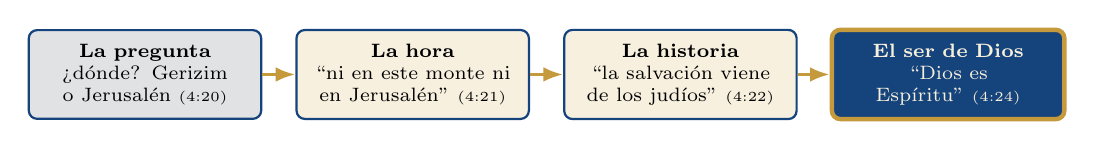
\begin{tikzpicture}[font=\scriptsize]
 \node[caja,text width=2.6cm,align=center,fill=gris!18] (a) at (0,0) {\textbf{La pregunta}\\ ¿dónde? Gerizim o Jerusalén {\tiny(4:20)}};
 \node[caja,text width=2.6cm,align=center] (b) at (3.4,0) {\textbf{La hora}\\ ``ni en este monte ni en Jerusalén'' {\tiny(4:21)}};
 \node[caja,text width=2.6cm,align=center] (c) at (6.8,0) {\textbf{La historia}\\ ``la salvación viene de los judíos'' {\tiny(4:22)}};
 \node[draw=dorado,line width=1.6pt,fill=azul,text=papiro,rounded corners=3pt,text width=2.6cm,align=center,inner sep=5pt] (d) at (10.2,0) {\textbf{El ser de Dios}\\ ``Dios es Espíritu'' {\tiny(4:24)}};
 \draw[-{Latex[length=2.5mm]},dorado,line width=1.2pt] (a)--(b); \draw[-{Latex[length=2.5mm]},dorado,line width=1.2pt] (b)--(c); \draw[-{Latex[length=2.5mm]},dorado,line width=1.2pt] (c)--(d);
\end{tikzpicture}\par\medskip
\begin{columns}[t,onlytextwidth]
\begin{column}{0.52\textwidth}\small
\begin{itemize}
\item Jesús no relativiza la revelación: ``nosotros adoramos lo que sabemos'' (4:22). La salvación tiene historia y pueblo.
\item Pero el Dios de esa historia no está atado a un monte. Lo que estaba ligado a un lugar se liga ahora a una persona y a una manera.
\item El Padre ``\destacar{busca}'' adoradores (\grc{ζητεῖ}): la iniciativa es suya.
\end{itemize}
\end{column}
\begin{column}{0.46\textwidth}
\begin{cita}Pero ¿es verdad que Dios morará sobre la tierra? He aquí que los cielos, los cielos de los cielos, no te pueden contener; ¿cuánto menos esta casa que yo he edificado?\fuente{(1 R 8:27, RVR1960)}\end{cita}
\scriptsize Salomón ya lo dijo al dedicar el templo.
\end{column}
\end{columns}
\end{frame}

\begin{frame}{``En espíritu y en verdad''}
\scriptsize\renewcommand{\arraystretch}{1.2}
\begin{tabular}{@{}>{\RaggedRight\arraybackslash}p{2.6cm}>{\RaggedRight\arraybackslash}p{4.6cm}>{\RaggedRight\arraybackslash}p{4.6cm}@{}}
\toprule
\textbf{Lectura} & \textbf{Sentido} & \textbf{Apoyo} \\ \midrule
Espíritu humano & adorar desde lo interior, no solo con ritos y lugares & MacArthur (nota a Jn 4:24); Is 66:2: ``humilde de espíritu'' \\
Espíritu Santo & adorar movidos por el Espíritu que Jesús dará & Jn 3:5--6; 7:38--39: el agua viva ``dijo del Espíritu'' \\
``Verdad'' & conforme a la revelación, centrada en Jesús & Jn 1:14, 17; 14:6 \\
\bottomrule
\end{tabular}\par\medskip
\begin{columns}[t,onlytextwidth]
\begin{column}{0.52\textwidth}
\begin{cita}mas el que bebiere del agua que yo le daré, no tendrá sed jamás; sino que el agua que yo le daré será en él una fuente de agua que salte para vida eterna.\fuente{(Jn 4:14, RVR1960)}\end{cita}
\end{column}
\begin{column}{0.46\textwidth}\small
La adoración ``en espíritu'' corresponde a lo que Dios \destacar{es}: el adorador debe ser semejante al adorado. Por eso el agua viva (4:14) y la adoración nueva (4:24) van juntas.
\end{column}
\end{columns}
\precision{la referencia de ``espíritu'' (humano o Espíritu Santo) se discute; el contexto de Juan (agua viva = Espíritu, 7:39) favorece que el espíritu humano adore movido por el Espíritu de Dios. Lectura propia.}
\end{frame}

% ------------------------------------------------------------------
\section{La palabra}

\begin{frame}{\emph{Rúaj}: viento, aliento, espíritu}
\centering
\begin{tikzpicture}[font=\scriptsize]
 \node[draw=dorado,line width=1.6pt,fill=azul,text=papiro,circle,minimum size=1.7cm,align=center] (c) at (0,0) {\heb{רוּחַ}\\ \emph{rúaj}};
 \node[caja,text width=3.0cm,align=center] (v) at (-4.3,1.2) {\textbf{Viento}\\ ``por recio viento oriental'' {\tiny(Éx 14:21)}};
 \node[caja,text width=3.0cm,align=center] (a) at (4.3,1.2) {\textbf{Aliento}\\ ``por el aliento de su boca'' {\tiny(Sal 33:6, \heb{וּבְרוּחַ פִּיו})}};
 \node[caja,text width=3.0cm,align=center] (h) at (-4.3,-1.3) {\textbf{Vida, ánimo}\\ ``el espíritu vuelva a Dios que lo dio'' {\tiny(Ec 12:7)}};
 \node[caja,text width=3.0cm,align=center] (e) at (4.3,-1.3) {\textbf{Espíritu de Dios}\\ ``el Espíritu de Dios se movía'' {\tiny(Gn 1:2)}};
 \foreach \i in {v,a,h,e}\draw[dorado,line width=1.1pt] (c)--(\i);
\end{tikzpicture}\par\medskip
\small\RaggedRight Lo común a todos los sentidos: algo \destacar{real, invisible y poderoso}. No se ve el viento, se ven sus efectos; no se ve el aliento, se ve la vida.\par\smallskip
\precision{Vine (1999) agrupa los usos en aliento, aire fugaz, viento, ánimo y espíritu; Chávez (1992) distingue ``espíritu, distinto e independiente del factor material'' (Pr 16:2; Is 31:3).}
\end{frame}

\begin{frame}{Gn 1:2 y Gn 2:7}
\begin{columns}[t,onlytextwidth]
\begin{column}{0.49\textwidth}
\begin{cita}Y la tierra estaba desordenada y vacía, y las tinieblas estaban sobre la faz del abismo, y el Espíritu de Dios se movía sobre la faz de las aguas.\fuente{(Gn 1:2, RVR1960)}\end{cita}
\begin{center}\heb{וְרוּחַ אֱלֹהִים מְרַחֶפֶת עַל־פְּנֵי הַמָּיִם}\end{center}
\scriptsize \heb{מְרַחֶפֶת} \emph{merajéfet}: ``se cernía'', como el águila sobre sus polluelos (\heb{יְרַחֵף}, Dt 32:11). La primera aparición de \emph{rúaj} es el Espíritu de Dios presente en la creación.
\end{column}
\begin{column}{0.49\textwidth}
\begin{cita}Entonces \SENOR{} Dios formó al hombre del polvo de la tierra, y sopló en su nariz aliento de vida, y fue el hombre un ser viviente.\fuente{(Gn 2:7, RVR1960)}\end{cita}
\begin{center}\heb{וַיִּפַּח בְּאַפָּיו נִשְׁמַת חַיִּים}\end{center}
\scriptsize \heb{נְשָׁמָה} \emph{neshamá}: ``aliento, hálito''. La RVR1960 la traduce ``espíritu'' en Job 26:4 y Pr 20:27: ``Lámpara de \SENOR{} es el espíritu del hombre''. El hombre vive porque Dios \destacar{sopla}.
\end{column}
\end{columns}\par\smallskip
\precision{la lectura de Gn 1:2 como ``viento de Dios'' (Ónkelos: \heb{וְרוּחָא מִן קֳדָם יְיָ מְנַשְּׁבָא}, ``un viento de delante del \SENOR{} soplaba'') es antigua; la RVR1960 lee ``Espíritu''.}
\end{frame}

\begin{frame}{El espectro completo: hebreo}
\scriptsize\renewcommand{\arraystretch}{1.12}
\begin{tabular}{@{}>{\RaggedRight\arraybackslash}p{2.8cm}>{\RaggedRight\arraybackslash}p{3.1cm}>{\RaggedRight\arraybackslash}p{3.0cm}>{\RaggedRight\arraybackslash}p{2.9cm}@{}}
\toprule
\textbf{Término} & \textbf{Sentido} & \textbf{RVR1960} & \textbf{Textos} \\ \midrule
\heb{רוּחַ} \emph{rúaj} (H7307) & viento, aliento, ánimo, espíritu & espíritu ($\approx$\,200), viento(s) ($\approx$\,74), aliento, soplo, hálito, aire, lado & Gn 1:2; 8:1; Nm 16:22; Is 31:3; Ez 37:9 \\
\heb{רוּחַ} \emph{rúaj} (arameo, H7308) & viento; espíritu, mente & espíritu, viento & Dn 2:35; 4:8; 5:12; 7:15 \\
\heb{נְשָׁמָה} \emph{neshamá} (H5397) & soplo, aliento vital & aliento, espíritu, soplo & Gn 2:7; Job 26:4; Pr 20:27 \\
\heb{נֶפֶשׁ} \emph{néfesh} & aliento, vida, persona & ``amargura de espíritu'' (\heb{מַר־נֶפֶשׁ}) & 1 S 22:2 \\
\bottomrule
\end{tabular}\par\medskip
\begin{columns}[t,onlytextwidth]
\begin{column}{0.49\textwidth}\scriptsize
\textbf{Conteo propio en la BHS:} \emph{rúaj} 376 veces en 349 versículos (366 en hebreo y 10 en arameo, con el etiquetado Strong incompleto). Vine da ``unas 378'' para el hebreo. Más frecuente en Ezequiel (51) e Isaías (49).
\end{column}
\begin{column}{0.49\textwidth}\scriptsize
\textbf{No es \emph{rúaj}:} \heb{רָוַח} (1 S 16:23, ``tenía alivio''), de la misma raíz \emph{r-w-ḥ} ``respirar, tener holgura''.
\end{column}
\end{columns}
\precision{los conteos por traducción salen de las etiquetas Strong de la RVR1960 y son aproximados; verificar en e-Sword.}
\end{frame}

\begin{frame}{El espectro completo: griego}
\scriptsize\renewcommand{\arraystretch}{1.12}
\begin{tabular}{@{}>{\RaggedRight\arraybackslash}p{2.7cm}>{\RaggedRight\arraybackslash}p{3.1cm}>{\RaggedRight\arraybackslash}p{2.9cm}>{\RaggedRight\arraybackslash}p{3.1cm}@{}}
\toprule
\textbf{Término} & \textbf{Sentido} & \textbf{RVR1960} & \textbf{Textos} \\ \midrule
\grc{πνεῦμα} (379) & viento, aliento, espíritu, Espíritu & espíritu, viento, aliento & Jn 3:8; 4:24; Ro 8:16; 2 Ts 2:8 \\
\grc{πνευματικός} (26) & espiritual & espiritual(es) & Ro 7:14; 1 Co 2:13--15; 15:44 \\
\grc{πνευματικῶς} (2) & espiritualmente & espiritualmente, en sentido espiritual & 1 Co 2:14; Ap 11:8 \\
\grc{πνοή} (2) & soplo, aliento & viento, aliento & Hch 2:2; 17:25 \\
\grc{πνέω} (7) & soplar & soplar & Jn 3:8; Hch 27:40 \\
\grc{ἐκπνέω} (3) & expirar & expirar & Mr 15:37; Lc 23:46 \\
\grc{θεόπνευστος} (1) & ``soplada por Dios'' & inspirada por Dios & 2 Ti 3:16 \\
\bottomrule
\end{tabular}\par\medskip
\small\RaggedRight La LXX traduce \emph{rúaj} casi siempre con \grc{πνεῦμα}. Jesús juega con el doble sentido: ``El viento (\grc{τὸ πνεῦμα}) sopla de donde quiere\ldots{} así es todo aquel que es nacido del Espíritu (\grc{ἐκ τοῦ πνεύματος})'' (Jn 3:8).\par\smallskip
\precision{\grc{φάντασμα} (``fantasma'', Mt 14:26; Mr 6:49) no se traduce ``espíritu''. En Lc 24:37 la RVR1960 traduce \grc{πνεῦμα} ``espíritu''.}
\end{frame}

\begin{frame}{Carne y no espíritu}
\begin{columns}[c,onlytextwidth]
\begin{column}{0.52\textwidth}
\begin{cita}Y los egipcios hombres son, y no Dios; y sus caballos carne, y no espíritu; de manera que al extender \SENOR{} su mano, caerá el ayudador y caerá el ayudado, y todos ellos desfallecerán a una.\fuente{(Is 31:3, RVR1960)}\end{cita}
\begin{center}\heb{וּמִצְרַיִם אָדָם וְלֹא־אֵל}\\[2pt]\heb{וְסוּסֵיהֶם בָּשָׂר וְלֹא־רוּחַ}\end{center}
\end{column}
\begin{column}{0.46\textwidth}
\centering
\begin{tikzpicture}[font=\scriptsize]
 \node[caja,text width=1.9cm,align=center,fill=gris!18] (a) at (0,1.2) {\heb{אָדָם} hombre};
 \node[draw=dorado,line width=1.4pt,fill=azul,text=papiro,rounded corners=3pt,text width=1.9cm,align=center,inner sep=4pt] (b) at (2.9,1.2) {\heb{אֵל} Dios};
 \node[caja,text width=1.9cm,align=center,fill=gris!18] (c) at (0,-0.2) {\heb{בָּשָׂר} carne};
 \node[draw=dorado,line width=1.4pt,fill=azul,text=papiro,rounded corners=3pt,text width=1.9cm,align=center,inner sep=4pt] (d) at (2.9,-0.2) {\heb{רוּחַ} espíritu};
 \draw[<->,gris,thick] (a)--(b) node[midway,above,font=\tiny]{no es}; \draw[<->,gris,thick] (c)--(d) node[midway,above,font=\tiny]{no es};
\end{tikzpicture}\par\smallskip
\RaggedRight\small Paralelismo: hombre // carne; Dios // espíritu. Judá confiaba en los caballos de Egipto (31:1); Isaías opone la \destacar{carne} perecedera al \destacar{espíritu} que pertenece a Dios.
\end{column}
\end{columns}\par\smallskip
\precision{(textual) la LXX no tiene ``y no espíritu'': lee \grc{καὶ οὐκ ἔστιν βοήθεια}, ``y no hay ayuda''. El Targum conserva \heb{בְּסַר וְלָא רוּחַ}.}
\end{frame}

\begin{frame}{Los ídolos: sin espíritu}
\begin{columns}[t,onlytextwidth]
\begin{column}{0.50\textwidth}
\begin{cita}Todo hombre se embrutece, y le falta ciencia; se avergüenza de su ídolo todo fundidor, porque mentirosa es su obra de fundición, y no hay espíritu en ella.\fuente{(Jer 10:14, RVR1960)}\end{cita}
\begin{cita}He aquí está cubierto de oro y plata, y no hay espíritu dentro de él.\fuente{(Hab 2:19b, RVR1960)}\end{cita}
\end{column}
\begin{column}{0.48\textwidth}\small
\begin{itemize}
\item \heb{וְלֹא־רוּחַ בָּם} (Jer 10:14), \heb{וְכָל־רוּחַ אֵין בְּקִרְבּוֹ} (Hab 2:19): el ídolo tiene forma y no tiene \emph{rúaj}.
\item Sal 135:17: ``Tampoco hay aliento (\heb{רוּחַ}) en sus bocas''.
\item El Dios verdadero es lo opuesto: no tiene forma visible y es \destacar{todo vida}.
\end{itemize}
\precision{Jer 10:14 pertenece al texto ancla del atributo Verdad (Jer 10:1--16): el ídolo es mentira porque no tiene espíritu.}
\end{column}
\end{columns}
\end{frame}

% ------------------------------------------------------------------
\section{El Nombre}

\begin{frame}{``Dios de los espíritus''}
\fotolado{panel_numeros16.jpg}{Elaboración propia: Nm 16:22 en texto hebreo consonántico (BHS).}
\begin{columns}[c,onlytextwidth]
\begin{column}{0.58\textwidth}
\begin{cita}Y ellos se postraron sobre sus rostros, y dijeron: Dios, Dios de los espíritus de toda carne, ¿no es un solo hombre el que pecó? ¿Por qué airarte contra toda la congregación?\fuente{(Nm 16:22, RVR1960)}\end{cita}
\begin{cita}Ponga \SENOR, Dios de los espíritus de toda carne, un varón sobre la congregación.\fuente{(Nm 27:16, RVR1960)}\end{cita}
\end{column}
\begin{column}{0.40\textwidth}\end{column}
\end{columns}
\end{frame}

\begin{frame}{Nm 16:22 y 27:16: filología}
\begin{center}\heb{אֵל אֱלֹהֵי הָרוּחֹת לְכָל־בָּשָׂר}\end{center}
\scriptsize\renewcommand{\arraystretch}{1.12}
\begin{tabular}{@{}>{\RaggedRight\arraybackslash}p{2.8cm}>{\RaggedRight\arraybackslash}p{9.0cm}@{}}
\toprule
\heb{אֵל אֱלֹהֵי} & ``Dios, Dios de\ldots'': vocativo doble en la oración de Moisés y Aarón. \\
\heb{הָרוּחֹת} \emph{harujot} & ``los espíritus'', plural de \emph{rúaj}: el aliento vital de cada ser humano. \\
\heb{לְכָל־בָּשָׂר} & ``de toda carne'': toda criatura viviente. \\
LXX & \grc{θεὸς θεὸς τῶν πνευμάτων καὶ πάσης σαρκός}: ``Dios de los espíritus \destacar{y} de toda carne''. \\
Ónkelos & \heb{אֵל אֱלָהּ רוּחַיָּא לְכָל בִּשְׂרָא}: conserva la fórmula. \\
\bottomrule
\end{tabular}\par\medskip
\begin{columns}[t,onlytextwidth]
\begin{column}{0.52\textwidth}\small
Las dos veces la fórmula aparece en una \destacar{oración}: Moisés apela al Dios que conoce cada espíritu, en el juicio (Coré) y en la sucesión (Josué).
\end{column}
\begin{column}{0.46\textwidth}\scriptsize
\textbf{Rashi} (Nm 16:22): \heb{יוֹדֵעַ מַחֲשָׁבוֹת}, ``conoce los pensamientos''; un rey de carne y sangre castiga a todos porque no sabe quién pecó; ``pero tú, ante ti están revelados todos los pensamientos''.\par\smallskip
\precision{comentario rabínico medieval (Sefaria); traducción propia.}
\end{column}
\end{columns}
\end{frame}

\begin{frame}{El Nombre que revela su ser espiritual}
\begin{columns}[c,onlytextwidth]
\begin{column}{0.44\textwidth}
\begin{cita}Profecía de la palabra de \SENOR{} acerca de Israel. \SENOR, que extiende los cielos y funda la tierra, y forma el espíritu del hombre dentro de él, ha dicho:\fuente{(Zac 12:1, RVR1960)}\end{cita}
\begin{cita}[fontupper=\scriptsize\itshape]¿Por qué no obedeceremos mucho mejor al Padre de los espíritus, y viviremos?\fuente{(He 12:9b, RVR1960)}\end{cita}
\end{column}
\begin{column}{0.54\textwidth}\scriptsize
\renewcommand{\arraystretch}{1.12}
\begin{tabular}{@{}>{\RaggedRight\arraybackslash}p{2.4cm}>{\RaggedRight\arraybackslash}p{2.5cm}>{\RaggedRight\arraybackslash}p{1.5cm}@{}}
\toprule
\textbf{Nombre} & \textbf{Original} & \textbf{Texto} \\ \midrule
Dios de los espíritus de toda carne & \heb{אֱלֹהֵי הָרוּחֹת לְכָל־בָּשָׂר} & Nm 16:22; 27:16 \\
El que forma el espíritu del hombre & \heb{יֹצֵר רוּחַ־אָדָם} & Zac 12:1 \\
El que da aliento y espíritu & \heb{נֹתֵן נְשָׁמָה}\ldots{} \heb{וְרוּחַ} & Is 42:5 \\
Padre de los espíritus & \grc{τῷ πατρὶ τῶν πνευμάτων} & He 12:9 \\
Dios de los espíritus de los profetas & \grc{ὁ θεὸς τῶν πνευμάτων τῶν προφητῶν} & Ap 22:6 \\
El Invisible & \grc{τὸν ἀόρατον} & He 11:27 \\
\bottomrule
\end{tabular}
\end{column}
\end{columns}\par\smallskip
\precision{no hay un nombre propio ``Espíritu'' en el AT; se usa el título ``Dios de los espíritus'', que lo revela como fuente y dueño de todo espíritu. El Nombre que revela el atributo es, en esta serie, Nm 16:22.}
\end{frame}

% ------------------------------------------------------------------
\section{Definición}

\begin{frame}{¿Qué significa ``Dios es Espíritu''?}
\begin{columns}[c,onlytextwidth]
\begin{column}{0.48\textwidth}
\begin{tcolorbox}[colback=papiro,colframe=azul,boxrule=1pt,arc=3pt,title={\small Definición},colbacktitle=azul,coltitle=papiro]
\small Que Dios es Espíritu es la perfección eterna de su \destacar{ser} por la cual Dios existe sin cuerpo, sin partes y sin forma visible; es vida en sí mismo y fuente de toda vida; no está limitado por lugar ni puede ser representado por imagen; y se da a conocer por su \destacar{palabra}, por su Espíritu y, en plenitud, en el \destacar{Hijo} hecho carne.
\end{tcolorbox}
\precision{definición de síntesis de esta serie, a partir de los textos estudiados.}
\end{column}
\begin{column}{0.50\textwidth}
\scriptsize\renewcommand{\arraystretch}{1.15}
\begin{tabular}{@{}>{\RaggedRight\arraybackslash}p{2.0cm}>{\RaggedRight\arraybackslash}p{4.2cm}@{}}
\toprule
\textbf{Rasgo} & \textbf{Texto} \\ \midrule
Incorpóreo & ``un espíritu no tiene carne ni huesos'' (Lc 24:39) \\
Invisible & ``Rey de los siglos, inmortal, invisible'' (1 Ti 1:17) \\
Vivo y vivificante & ``El espíritu es el que da vida'' (Jn 6:63) \\
Sin límite de lugar & ``¿A dónde me iré de tu Espíritu?'' (Sal 139:7) \\
Sin imagen & ``ninguna figura visteis'' (Dt 4:15) \\
Personal & ``el Padre tales adoradores busca'' (Jn 4:23) \\
\bottomrule
\end{tabular}
\end{column}
\end{columns}
\end{frame}

\begin{frame}{Lo que no significa}
\scriptsize\renewcommand{\arraystretch}{1.2}
\begin{tabular}{@{}>{\RaggedRight\arraybackslash}p{3.5cm}>{\RaggedRight\arraybackslash}p{8.3cm}@{}}
\toprule
\textbf{Malentendido} & \textbf{Respuesta bíblica} \\ \midrule
``Un espíritu entre otros'' & Es ``Padre de los espíritus'' (He 12:9); los demás espíritus son criaturas (Zac 12:1). \\
Fuerza impersonal, energía & Habla, busca, ama: ``el Padre tales adoradores busca'' (Jn 4:23). \\
Irreal, vago, lejano & Es lo más real: lo visible es temporal; ``las que no se ven son eternas'' (2 Co 4:18). \\
Hostil a lo material & Creó la materia y la llamó buena (Gn 1:31); en Cristo habita ``corporalmente'' (Col 2:9). \\
Solo ``el Espíritu Santo'' & ``Dios es Espíritu'' dice qué es Dios (Padre, Hijo y Espíritu); ``el Espíritu Santo'' es una de las personas. \\
\bottomrule
\end{tabular}\par\medskip
\begin{tcolorbox}[colback=papiro,colframe=dorado,boxrule=1.2pt,arc=3pt]
\small ``Debido a que es `espíritu', es incorpóreo, no tiene sustancia visible. Si Dios tuviera un cuerpo tangible, no sería omnipresente\ldots; pero precisamente porque es `espíritu', llena el cielo y la tierra'' (Pink, 2020, cap. 16).
\end{tcolorbox}
\end{frame}

\begin{frame}{Manos, ojos, alas: el lenguaje de los hombres}
\begin{columns}[t,onlytextwidth]
\begin{column}{0.50\textwidth}\scriptsize\renewcommand{\arraystretch}{1.15}
\begin{tabular}{@{}>{\RaggedRight\arraybackslash}p{1.7cm}>{\RaggedRight\arraybackslash}p{3.9cm}@{}}
\toprule
\textbf{Imagen} & \textbf{Texto} \\ \midrule
Mano & ``al extender \SENOR{} su mano'' (Is 31:3) \\
Ojos & ``los ojos de \SENOR{} contemplan toda la tierra'' (2 Cr 16:9) \\
Alas & ``bajo sus alas estarás seguro'' (Sal 91:4) \\
Trono & ``El cielo es mi trono'' (Is 66:1) \\
\bottomrule
\end{tabular}\par\smallskip
\small La Biblia describe a Dios con imágenes del cuerpo (\emph{antropomorfismos}) para hablar de su poder, su cuidado y su gobierno.
\end{column}
\begin{column}{0.48\textwidth}\small
\begin{itemize}
\item Los sabios lo resumen así: \heb{דִּבְּרָה תוֹרָה כִּלְשׁוֹן בְּנֵי אָדָם}, ``la Torá habló en el lenguaje de los hombres'' (Berajot 31b, citado por Maimónides).
\item Las imágenes son verdaderas como \destacar{imágenes}: Dios realmente actúa, ve y protege; pero no tiene miembros.
\item La misma Torá que dice ``mano'' prohíbe hacer una figura de Dios (Dt 4:15--16).
\end{itemize}
\end{column}
\end{columns}\par\smallskip
\precision{el principio rabínico se cita según Maimónides, \emph{Mishné Torá}, Yesodé haTorá 1:9 y su comentario a la Misná, Sanedrín 10:1 (Sefaria).}
\end{frame}

% ------------------------------------------------------------------
\section{Teología}

\begin{frame}{Invisible, pero revelado}
\begin{columns}[t,onlytextwidth]
\begin{column}{0.50\textwidth}
\begin{cita}Dijo más: No podrás ver mi rostro; porque no me verá hombre, y vivirá.\fuente{(Éx 33:20, RVR1960)}\end{cita}
\begin{cita}el único que tiene inmortalidad, que habita en luz inaccesible; a quien ninguno de los hombres ha visto ni puede ver, al cual sea la honra y el imperio sempiterno. Amén.\fuente{(1 Ti 6:16, RVR1960)}\end{cita}
\end{column}
\begin{column}{0.48\textwidth}\small
\begin{itemize}
\item Ningún ser humano ``ha visto ni puede ver'' a Dios: no por distancia, sino por lo que Dios \destacar{es}.
\item Pink: Dios ``sólo puede ser conocido espiritualmente''; el conocimiento salvador viene cuando el Espíritu ilumina el corazón (2 Co 4:6) (Pink, 2020, cap. 1).
\item El Dios invisible \destacar{habla}: Moisés no vio su rostro, pero oyó su Nombre (Éx 34:5--7).
\end{itemize}
\end{column}
\end{columns}
\precision{la autoría paulina de 1 Timoteo se discute; la misma idea aparece en cartas indiscutidas: ``las cosas invisibles de él'' (Ro 1:20).}
\end{frame}

\begin{frame}{Espíritu y presencia}
\begin{columns}[c,onlytextwidth]
\begin{column}{0.50\textwidth}
\begin{cita}¿A dónde me iré de tu Espíritu? ¿Y a dónde huiré de tu presencia? Si subiere a los cielos, allí estás tú; Y si en el Seol hiciere mi estrado, he aquí, allí tú estás.\fuente{(Sal 139:7--8, RVR1960)}\end{cita}
\begin{center}\heb{אָנָה אֵלֵךְ מֵרוּחֶךָ וְאָנָה מִפָּנֶיךָ אֶבְרָח}\end{center}
\end{column}
\begin{column}{0.48\textwidth}\small
\begin{itemize}
\item Paralelismo: ``tu Espíritu'' // ``tu presencia'' (\heb{פָּנֶיךָ}, ``tu rostro'').
\item Porque es Espíritu, Dios no ocupa un lugar: \destacar{está} en todo lugar. Este rasgo se estudiará en el atributo \emph{Omnipresente}.
\item Lo que en Jn 4 suprime el monte, en el Salmo 139 suprime la huida.
\end{itemize}
\end{column}
\end{columns}
\end{frame}

\begin{frame}{Espíritu que da vida}
\begin{columns}[t,onlytextwidth]
\begin{column}{0.50\textwidth}
\begin{cita}Y me dijo: Profetiza al espíritu, profetiza, hijo de hombre, y dí al espíritu: Así ha dicho \SENOR{} el Señor: Espíritu, ven de los cuatro vientos, y sopla sobre estos muertos, y vivirán.\fuente{(Ez 37:9, RVR1960)}\end{cita}
\begin{center}\heb{מֵאַרְבַּע רוּחוֹת בֹּאִי הָרוּחַ}\end{center}
\scriptsize ``De los cuatro \emph{rujot} ven, \emph{rúaj}'': viento, aliento y Espíritu en una sola frase. En 37:14 Dios dice: ``pondré mi Espíritu (\heb{רוּחִי}) en vosotros, y viviréis''.
\end{column}
\begin{column}{0.48\textwidth}\small
\begin{itemize}
\item El Dios que es Espíritu es \destacar{vivo} y da vida: Gn 2:7; Ez 37; Jn 6:63.
\item ``El espíritu es el que da vida; la carne para nada aprovecha'' (Jn 6:63).
\item Los ídolos no tienen \emph{rúaj} (Jer 10:14); el Dios vivo la \destacar{da}.
\end{itemize}
\end{column}
\end{columns}
\end{frame}

\begin{frame}{Un reflejo en el ser humano}
\begin{columns}[t,onlytextwidth]
\begin{column}{0.50\textwidth}
\begin{cita}Porque ¿quién de los hombres sabe las cosas del hombre, sino el espíritu del hombre que está en él? Así tampoco nadie conoció las cosas de Dios, sino el Espíritu de Dios.\fuente{(1 Co 2:11, RVR1960)}\end{cita}
\begin{cita}y el polvo vuelva a la tierra, como era, y el espíritu vuelva a Dios que lo dio.\fuente{(Ec 12:7, RVR1960)}\end{cita}
\end{column}
\begin{column}{0.48\textwidth}\small
\begin{itemize}
\item Dios \destacar{dio} espíritu al ser humano (Gn 2:7; Zac 12:1; Ec 12:7): por eso el atributo es comunicable como reflejo.
\item Pablo usa la analogía: como el espíritu del hombre conoce lo íntimo del hombre, solo el Espíritu de Dios conoce lo íntimo de Dios.
\item Pero el espíritu humano es \destacar{dado}, limitado y unido a un cuerpo; el de Dios es increado.
\end{itemize}
\end{column}
\end{columns}\par\smallskip
\precision{1 Co 2:10--11 es el texto que el libro usa como marco de humildad: lo profundo de Dios solo lo conoce su Espíritu.}
\end{frame}

% ------------------------------------------------------------------
\section{En Israel}

\begin{frame}{Horeb: una voz sin figura}
\fotolado{panel_deuteronomio4.jpg}{Elaboración propia: Dt 4:12 en texto hebreo consonántico (BHS).}
\begin{columns}[c,onlytextwidth]
\begin{column}{0.58\textwidth}
\begin{cita}y habló \SENOR{} con vosotros de en medio del fuego; oísteis la voz de sus palabras, mas a excepción de oír la voz, ninguna figura visteis.\fuente{(Dt 4:12, RVR1960)}\end{cita}
\begin{cita}Guardad, pues, mucho vuestras almas; pues ninguna figura visteis el día que \SENOR{} habló con vosotros de en medio del fuego;\fuente{(Dt 4:15, RVR1960)}\end{cita}
\end{column}
\begin{column}{0.40\textwidth}\end{column}
\end{columns}
\end{frame}

\begin{frame}{Dt 4:12--19 en hebreo}
\begin{center}\heb{קוֹל דְּבָרִים אַתֶּם שֹׁמְעִים וּתְמוּנָה אֵינְכֶם רֹאִים זוּלָתִי קוֹל}\end{center}
\scriptsize\renewcommand{\arraystretch}{1.12}
\begin{tabular}{@{}>{\RaggedRight\arraybackslash}p{2.8cm}>{\RaggedRight\arraybackslash}p{1.1cm}>{\RaggedRight\arraybackslash}p{7.9cm}@{}}
\toprule
\textbf{Término} & \textbf{Raíz} & \textbf{Sentido} \\ \midrule
\heb{קוֹל דְּבָרִים} & \heb{קול} & ``voz de palabras'': Israel recibió \destacar{palabras}, no una imagen. \\
\heb{תְּמוּנָה} \emph{temuná} & \heb{מין} & ``figura, forma visible''. Lo que Israel \destacar{no} vio. \\
\heb{פֶּסֶל} \emph{pésel} & \heb{פסל} & ``escultura, imagen tallada'' (4:16). \\
\heb{סֶמֶל} \emph{sémel} & --- & ``efigie, estatua'' (4:16). \\
\heb{תַּבְנִית} \emph{tavnit} & \heb{בנה} & ``figura, modelo'': de varón, hembra, animal, ave, reptil, pez (4:16--18). \\
LXX 4:12 & --- & \grc{ὁμοίωμα οὐκ εἴδετε ἀλλ’ ἢ φωνήν}: ``semejanza no visteis, sino una voz''. \\
\bottomrule
\end{tabular}\par\medskip
\small\RaggedRight Moisés saca la consecuencia: como no hubo figura, \destacar{no se hará figura}. La forma de la revelación (voz sin imagen) corresponde al ser de Dios (Espíritu sin cuerpo).
\end{frame}

\begin{frame}{El becerro y la voz}
\centering
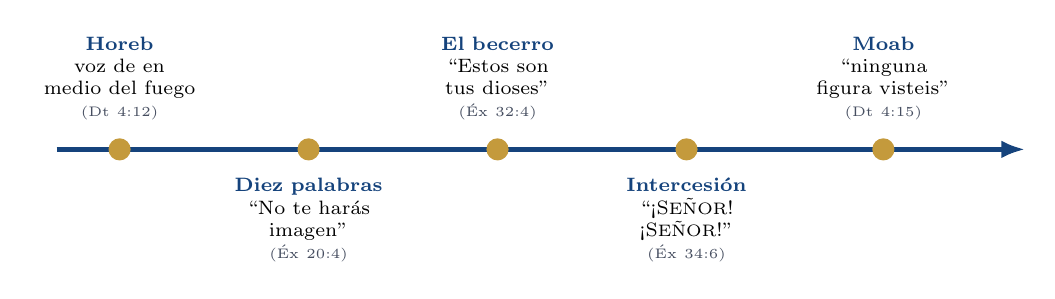
\begin{tikzpicture}[font=\scriptsize]
 \draw[line width=1.6pt,azul,-{Latex[length=3mm]}] (-0.3,0) -- (12.0,0);
 \foreach \x/\t/\b/\r/\pos in {0.5/{Horeb}/{voz de en medio del fuego}/{Dt 4:12}/above,
   2.9/{Diez palabras}/{``No te harás imagen''}/{Éx 20:4}/below,
   5.3/{El becerro}/{``Estos son tus dioses''}/{Éx 32:4}/above,
   7.7/{Intercesión}/{``¡\SENOR! ¡\SENOR!''}/{Éx 34:6}/below,
   10.2/{Moab}/{``ninguna figura visteis''}/{Dt 4:15}/above}{
  \fill[dorado] (\x,0) circle (4pt);
  \node[\pos=7pt,text width=2.1cm,align=center] at (\x,0) {\textbf{\textcolor{azul}{\t}}\\ \b\\ {\tiny\color{gris}(\r)}};}
\end{tikzpicture}\par\medskip
\begin{columns}[t,onlytextwidth]
\begin{column}{0.49\textwidth}\small
\begin{itemize}
\item En Horeb Dios se reveló como \destacar{voz}. Al pie del monte, Israel quiso un dios que se \destacar{viera}.
\item Cuarenta años después, en Moab, Moisés recuerda la escena a la nueva generación: la idolatría empieza por querer ver.
\end{itemize}
\end{column}
\begin{column}{0.49\textwidth}
\begin{cita}y cambiaron su gloria Por la imagen de un buey que come hierba.\fuente{(Sal 106:20, RVR1960)}\end{cita}
\end{column}
\end{columns}
\end{frame}

\begin{frame}{Dt 4:16--18: la lista de figuras}
\scriptsize\renewcommand{\arraystretch}{1.18}
\begin{tabular}{@{}>{\RaggedRight\arraybackslash}p{3.1cm}>{\RaggedRight\arraybackslash}p{4.3cm}>{\RaggedRight\arraybackslash}p{4.4cm}@{}}
\toprule
\textbf{Dt 4:16--18} & \textbf{LXX} & \textbf{Ro 1:23} \\ \midrule
figura, efigie & \grc{ὁμοίωμα}, \grc{εἰκών} & \grc{ἐν ὁμοιώματι εἰκόνος} \\
varón o hembra & \grc{ἀρσενικοῦ ἢ θηλυκοῦ} & \grc{φθαρτοῦ ἀνθρώπου} \\
animal de la tierra & \grc{κτήνους} & \grc{τετραπόδων} \\
ave alada & \grc{ὀρνέου πτερωτοῦ} & \grc{πετεινῶν} \\
lo que se arrastra & \grc{ἑρπετοῦ} & \grc{ἑρπετῶν} \\
\bottomrule
\end{tabular}\par\medskip
\begin{columns}[t,onlytextwidth]
\begin{column}{0.52\textwidth}
\begin{cita}y cambiaron la gloria del Dios incorruptible en semejanza de imagen de hombre corruptible, de aves, de cuadrúpedos y de reptiles.\fuente{(Ro 1:23, RVR1960)}\end{cita}
\end{column}
\begin{column}{0.46\textwidth}\small
Pablo describe la idolatría humana con el vocabulario de Dt 4 y del Sal 106:20 (``cambiaron su gloria'', LXX \grc{ἠλλάξαντο τὴν δόξαν}). Lo que Horeb prohibió, el mundo lo hizo.
\end{column}
\end{columns}
\precision{el eco de Dt 4:16--18 y Sal 106:20 en Ro 1:23 es lectura de varios intérpretes (cf. Dunn, 1998); se apoya en el vocabulario común de la LXX.}
\end{frame}

% ------------------------------------------------------------------
\section{Judaísmo}

\begin{frame}{El alma y el Santo}
\begin{columns}[t,onlytextwidth]
\begin{column}{0.50\textwidth}\small
\emph{Berajot} 10a: ¿por qué David dijo cinco veces ``Bendice, alma mía, a \SENOR''? Rabí Yehoshúa ben Leví responde que el \destacar{alma} se parece al \destacar{Santo}:
\begin{center}\scriptsize\heb{מָה הַקָּדוֹשׁ בָּרוּךְ הוּא רוֹאֶה וְאֵינוֹ נִרְאֶה}\\ \heb{אַף נְשָׁמָה רוֹאָה וְאֵינָהּ נִרְאֵית}\end{center}
``Como el Santo, bendito sea, ve y no es visto, así el alma ve y no es vista''.
\end{column}
\begin{column}{0.48\textwidth}\scriptsize\renewcommand{\arraystretch}{1.12}
\begin{tabular}{@{}>{\RaggedRight\arraybackslash}p{2.6cm}>{\RaggedRight\arraybackslash}p{2.8cm}@{}}
\toprule
\textbf{El Santo} & \textbf{El alma} \\ \midrule
llena todo el mundo & llena todo el cuerpo \\
ve y no es visto & ve y no es vista \\
sustenta el mundo & sustenta el cuerpo \\
es puro & es pura \\
mora en lo más íntimo & mora en lo más íntimo \\
\bottomrule
\end{tabular}\par\smallskip
``Venga quien tiene estas cinco cosas y alabe al que tiene estas cinco cosas''.
\end{column}
\end{columns}\par\smallskip
\precision{interpretación rabínica (Talmud de Babilonia, edición William Davidson, Sefaria); traducción propia. Es una analogía: el alma es criatura, Dios no.}
\end{frame}

\begin{frame}{Maimónides: ``no es cuerpo''}
\begin{columns}[t,onlytextwidth]
\begin{column}{0.52\textwidth}\scriptsize
\textbf{Tercer principio} (Comentario a la Misná, Sanedrín 10:1): ``la negación de la corporeidad'': Dios ``no es cuerpo ni fuerza en un cuerpo''. Se apoya en Dt 4:15: \heb{כִּי לֹא רְאִיתֶם כָּל תְּמוּנָה}.\par\smallskip
\textbf{\emph{Mishné Torá}, Yesodé haTorá 1:8}: \heb{שֶׁאֵין הַקָּדוֹשׁ בָּרוּךְ הוּא גּוּף וּגְוִיָּה}, ``el Santo, bendito sea, no es cuerpo ni figura''; y un cuerpo no puede estar en dos lugares.\par\smallskip
\textbf{Teshuvá 3:7}: entre los ``herejes'' (\emph{minim}) cuenta al que dice que hay un solo Señor, ``pero que es cuerpo y tiene figura''.
\end{column}
\begin{column}{0.46\textwidth}\scriptsize
\textbf{\emph{Yigdal}}, himno de la oración de la mañana basado en los trece principios:
\begin{center}\heb{אֵין לוֹ דְמוּת הַגּוּף וְאֵינוֹ גוּף}\end{center}
``No tiene semejanza de cuerpo, ni es cuerpo''.\par\smallskip
\textbf{\emph{Jaguigá} 15a} (citado por Maimónides): ``arriba no hay sentarse ni estar de pie''.\par\smallskip
\precision{lecturas judías medievales; \emph{Yigdal} se atribuye a Daniel ben Yehudá de Roma (siglo XIV). Textos según Sefaria; traducción propia.}
\end{column}
\end{columns}\par\medskip
\small\RaggedRight Para Maimónides, la incorporeidad de Dios es parte de la fe misma de Israel, no un detalle filosófico.
\end{frame}

\begin{frame}{\emph{Rúaj} en la \emph{Guía de los perplejos}}
\scriptsize\renewcommand{\arraystretch}{1.12}
\begin{tabular}{@{}>{\RaggedRight\arraybackslash}p{0.5cm}>{\RaggedRight\arraybackslash}p{4.4cm}>{\RaggedRight\arraybackslash}p{6.8cm}@{}}
\toprule
& \textbf{Sentido (Guía I:40)} & \textbf{Texto que cita} \\ \midrule
1 & el aire, uno de los cuatro elementos & ``el Espíritu de Dios se movía'' (Gn 1:2) \\
2 & el viento que sopla & ``el viento oriental trajo la langosta'' (Éx 10:13) \\
3 & el espíritu vital & ``soplo que va y no vuelve'' (Sal 78:39); Gn 7:15 \\
4 & lo que queda del hombre después de la muerte & ``el espíritu vuelva a Dios que lo dio'' (Ec 12:7) \\
5 & la influencia intelectual divina sobre los profetas & ``tomaré del espíritu que está en ti'' (Nm 11:17); 2 S 23:2 \\
6 & la intención, la voluntad & ``¿Quién enseñó al Espíritu de \SENOR?'' (Is 40:13) \\
\bottomrule
\end{tabular}\par\medskip
\begin{columns}[t,onlytextwidth]
\begin{column}{0.52\textwidth}\small
Maimónides abre: \heb{׳רוּחַ׳ שֵׁם מִשְׁתַּתֵּף}, ``\emph{rúaj} es un nombre equívoco'' (de varios sentidos). Todo \emph{rúaj} atribuido a Dios es, para él, el sentido 5 o el 6.
\end{column}
\begin{column}{0.46\textwidth}
\precision{versión hebrea de Samuel ibn Tibbon (Sefaria); traducción propia. Su lectura filosófica del Espíritu como ``influencia'' no coincide con la lectura cristiana del Espíritu como persona.}
\end{column}
\end{columns}
\end{frame}

\begin{frame}{Los targumes y Rashi}
\scriptsize\renewcommand{\arraystretch}{1.18}
\begin{tabular}{@{}>{\RaggedRight\arraybackslash}p{2.4cm}>{\RaggedRight\arraybackslash}p{9.4cm}@{}}
\toprule
\textbf{Ónkelos} (Éx 24:10) & El hebreo dice ``vieron al Dios de Israel''; Ónkelos: \heb{וַחֲזוֹ יָת יְקַר אֱלָהָא דְיִשְׂרָאֵל}, ``vieron \destacar{la gloria} del Dios de Israel''. \\
\textbf{Ónkelos} (Dt 4:12) & \heb{וּדְמוּת לֵיתֵיכוֹן חָזָן אֶלָּהֵן קָלָא}: ``y semejanza no veis, sino la voz''. \\
\textbf{Ónkelos} (Gn 1:2) & \heb{וְרוּחָא מִן קֳדָם יְיָ מְנַשְּׁבָא}: ``y un viento de delante del \SENOR{} soplaba''. \\
\textbf{Rashi} (Gn 1:2) & \heb{כִּסֵּא הַכָּבוֹד עוֹמֵד בָּאֲוִיר וּמְרַחֵף עַל פְּנֵי הַמַּיִם בְּרוּחַ פִּיו}: ``el trono de gloria estaba en el aire y se cernía sobre las aguas por el aliento de su boca'', ``como paloma que se cierne sobre el nido''. \\
\textbf{Rashi} (Nm 27:16) & ``Dios de los espíritus'': ``manifiesto ante ti es el pensamiento de cada uno, y no se parecen entre sí''; Moisés pide un guía que soporte a cada uno según su manera de pensar. \\
\bottomrule
\end{tabular}\par\medskip
\small\RaggedRight Los targumes evitan decir que alguien \destacar{vio} a Dios: ponen ``la gloria'' o ``la voz''. Es la misma convicción de Dt 4.\par\smallskip
\precision{interpretaciones judías antiguas y medievales (Sefaria); traducción propia.}
\end{frame}

\begin{frame}{Qumrán: espíritu y verdad}
\begin{columns}[t,onlytextwidth]
\begin{column}{0.52\textwidth}\small
La \emph{Regla de la Comunidad} (1QS) enseña que Dios puso en el hombre ``dos espíritus'', el de la \destacar{verdad} y el de la falsedad, hasta el tiempo de su visita (1QS III 17--19).\par\smallskip
Al final, Dios purificará al hombre con ``espíritu de santidad'' y ``rociará sobre él el espíritu de verdad como aguas de purificación'' (1QS IV 20--21).
\end{column}
\begin{column}{0.46\textwidth}
\centering
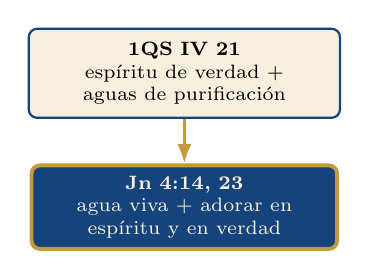
\begin{tikzpicture}[font=\scriptsize]
 \node[caja,text width=3.6cm,align=center] (a) at (0,1.3) {\textbf{1QS IV 21}\\ espíritu de verdad + aguas de purificación};
 \node[draw=dorado,line width=1.4pt,fill=azul,text=papiro,rounded corners=3pt,text width=3.6cm,align=center,inner sep=4pt] (b) at (0,-0.4) {\textbf{Jn 4:14, 23}\\ agua viva + adorar en espíritu y en verdad};
 \draw[-{Latex[length=2.5mm]},dorado,line width=1.1pt](a)--(b);
\end{tikzpicture}
\end{column}
\end{columns}\par\smallskip
\precision{paráfrasis según García Martínez (1992) y Vermes (2004); conviene cotejar en la Leon Levy Dead Sea Scrolls Digital Library. La relación con Juan es un paralelo de lenguaje, no una dependencia demostrada.}
\end{frame}

% ------------------------------------------------------------------
\section{En Cristo}

\begin{frame}{La imagen del Dios invisible}
\begin{columns}[t,onlytextwidth]
\begin{column}{0.50\textwidth}
\begin{cita}El es la imagen del Dios invisible, el primogénito de toda creación.\fuente{(Col 1:15, RVR1960)}\end{cita}
\begin{cita}Porque en él habita corporalmente toda la plenitud de la Deidad,\fuente{(Col 2:9, RVR1960)}\end{cita}
\end{column}
\begin{column}{0.48\textwidth}\scriptsize\renewcommand{\arraystretch}{1.12}
\begin{tabular}{@{}>{\RaggedRight\arraybackslash}p{2.2cm}>{\RaggedRight\arraybackslash}p{3.4cm}@{}}
\toprule
\grc{εἰκὼν τοῦ θεοῦ τοῦ ἀοράτου} & ``imagen del Dios \destacar{invisible}'' \\
\grc{κατοικεῖ} & ``habita'' de modo permanente \\
\grc{σωματικῶς} & ``\destacar{corporalmente}'' \\
\bottomrule
\end{tabular}\par\smallskip
\small La única ``imagen'' legítima de Dios no la hizo el hombre: es el Hijo. El Dios que es Espíritu, sin cuerpo, habita en plenitud en un \destacar{cuerpo}.
\end{column}
\end{columns}\par\smallskip
\precision{la autoría paulina de Colosenses se discute; la misma idea aparece en 2 Co 4:4: Cristo, ``el cual es la imagen de Dios''.}
\end{frame}

\begin{frame}{Dt 4 cumplido: Dios se deja ver}
\centering
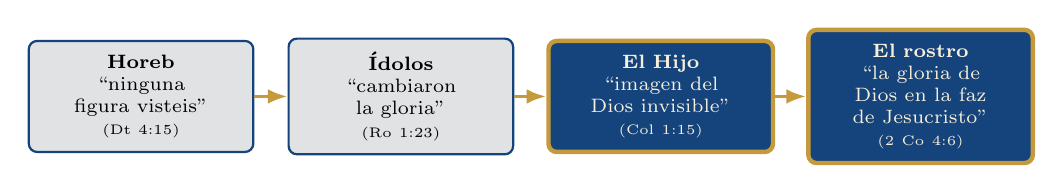
\begin{tikzpicture}[font=\scriptsize]
 \node[caja,text width=2.5cm,align=center,fill=gris!18] (a) at (0,0) {\textbf{Horeb}\\ ``ninguna figura visteis''\\ {\tiny(Dt 4:15)}};
 \node[caja,text width=2.5cm,align=center,fill=gris!18] (b) at (3.3,0) {\textbf{Ídolos}\\ ``cambiaron la gloria''\\ {\tiny(Ro 1:23)}};
 \node[draw=dorado,line width=1.6pt,fill=azul,text=papiro,rounded corners=3pt,text width=2.5cm,align=center,inner sep=5pt] (c) at (6.6,0) {\textbf{El Hijo}\\ ``imagen del Dios invisible''\\ {\tiny(Col 1:15)}};
 \node[draw=dorado,line width=1.6pt,fill=azul,text=papiro,rounded corners=3pt,text width=2.5cm,align=center,inner sep=5pt] (d) at (9.9,0) {\textbf{El rostro}\\ ``la gloria de Dios en la faz de Jesucristo''\\ {\tiny(2 Co 4:6)}};
 \draw[-{Latex[length=2.5mm]},dorado,line width=1.2pt] (a)--(b); \draw[-{Latex[length=2.5mm]},dorado,line width=1.2pt] (b)--(c); \draw[-{Latex[length=2.5mm]},dorado,line width=1.2pt] (c)--(d);
\end{tikzpicture}\par\medskip
\begin{columns}[t,onlytextwidth]
\begin{column}{0.52\textwidth}
\begin{cita}A Dios nadie le vio jamás; el unigénito Hijo, que está en el seno del Padre, él le ha dado a conocer.\fuente{(Jn 1:18, RVR1960)}\end{cita}
\scriptsize \grc{ἐξηγήσατο}: ``lo explicó, lo narró''. El Hijo es la exégesis del Padre.
\end{column}
\begin{column}{0.46\textwidth}\small
El que dijo ``no me verá hombre, y vivirá'' (Éx 33:20) se deja ver en el Hijo: ``El que me ha visto a mí, ha visto al Padre'' (Jn 14:9).\par\smallskip
\precision{(textual) en Jn 1:18 NA28 lee \grc{μονογενὴς θεός}, ``el unigénito Dios''; la RVR1960 sigue el texto bizantino \grc{ὁ μονογενὴς υἱός}, ``el unigénito Hijo''.}
\end{column}
\end{columns}
\end{frame}

\begin{frame}{``El Señor es el Espíritu''}
\fotolado{panel_2corintios3.jpg}{Elaboración propia: 2 Co 3:17 en escritura uncial (texto NA28), con \emph{nomina sacra}.}
\begin{columns}[c,onlytextwidth]
\begin{column}{0.58\textwidth}
\begin{cita}Pero cuando se conviertan al Señor, el velo se quitará. Porque el Señor es el Espíritu; y donde está el Espíritu del Señor, allí hay libertad. Por tanto, nosotros todos, mirando a cara descubierta como en un espejo la gloria del Señor, somos transformados de gloria en gloria en la misma imagen, como por el Espíritu del Señor.\fuente{(2 Co 3:16--18, RVR1960)}\end{cita}
\end{column}
\begin{column}{0.40\textwidth}\end{column}
\end{columns}
\end{frame}

\begin{frame}{2 Co 3:16--17 y Éx 34:34}
\scriptsize\renewcommand{\arraystretch}{1.15}
\begin{tabular}{@{}>{\RaggedRight\arraybackslash}p{1.6cm}>{\RaggedRight\arraybackslash}p{5.6cm}>{\RaggedRight\arraybackslash}p{4.6cm}@{}}
\toprule
\textbf{Texto} & \textbf{Original} & \textbf{RVR1960} \\ \midrule
Éx 34:34 TM & \heb{וּבְבֹא מֹשֶׁה לִפְנֵי יְהוָה}\ldots{} \heb{יָסִיר אֶת־הַמַּסְוֶה} & ``Cuando venía Moisés delante de \SENOR\ldots{} se quitaba el velo'' \\
Éx 34:34 LXX & \grc{ἡνίκα δ’ ἂν εἰσεπορεύετο Μωυσῆς ἔναντι κυρίου\ldots{} περιῃρεῖτο τὸ κάλυμμα} & --- \\
2 Co 3:16 & \grc{ἡνίκα δὲ ἐὰν ἐπιστρέψῃ πρὸς κύριον, περιαιρεῖται τὸ κάλυμμα} & ``cuando se conviertan al Señor, el velo se quitará'' \\
2 Co 3:17 & \grc{ὁ δὲ κύριος τὸ πνεῦμά ἐστιν} & ``el Señor es el Espíritu'' \\
\bottomrule
\end{tabular}\par\medskip
\begin{columns}[t,onlytextwidth]
\begin{column}{0.52\textwidth}\small
\begin{itemize}
\item Pablo cita Éx 34:34 casi palabra por palabra: el ``Señor'' (\grc{κύριος}) ante quien Moisés se quitaba el velo es el \SENOR{} del Sinaí.
\item Y explica: ese \SENOR{} se encuentra hoy ``en el Espíritu''. El velo se quita cuando uno se vuelve al Señor que es Espíritu.
\end{itemize}
\end{column}
\begin{column}{0.46\textwidth}
\precision{``el Señor es el Espíritu'' no confunde al Hijo con el Espíritu: es una exégesis de Éx 34 (``el Señor'' del texto se refiere al Espíritu que da vida, 3:6). Lectura sostenida por Dunn (1998) y Hays (1989).}
\end{column}
\end{columns}
\end{frame}

\begin{frame}{Pablo en Atenas}
\begin{columns}[t,onlytextwidth]
\begin{column}{0.50\textwidth}
\begin{cita}El Dios que hizo el mundo y todas las cosas que en él hay, siendo Señor del cielo y de la tierra, no habita en templos hechos por manos humanas, ni es honrado por manos de hombres, como si necesitase de algo; pues él es quien da a todos vida y aliento y todas las cosas.\fuente{(Hch 17:24--25, RVR1960)}\end{cita}
\end{column}
\begin{column}{0.48\textwidth}
\begin{cita}Siendo, pues, linaje de Dios, no debemos pensar que la Divinidad sea semejante a oro, o plata, o piedra, escultura de arte y de imaginación de hombres.\fuente{(Hch 17:29, RVR1960)}\end{cita}
\small Pablo predica a griegos con el lenguaje de Israel: \grc{οὐκ ἐν χειροποιήτοις ναοῖς}, ``no en templos hechos de mano'' (cf. 1 R 8:27; Is 66:1), y \grc{πνοή}, el ``aliento'' que Dios da (Gn 2:7; Is 42:5).
\end{column}
\end{columns}\par\smallskip
\precision{discurso transmitido por Lucas; lo usamos como testimonio de la predicación de Pablo.}
\end{frame}

\begin{frame}{El nuevo templo: ni Gerizim ni Jerusalén}
\begin{cita}porque por medio de él los unos y los otros tenemos entrada por un mismo Espíritu al Padre\ldots{} en quien vosotros también sois juntamente edificados para morada de Dios en el Espíritu.\fuente{(Ef 2:18, 22, RVR1960)}\end{cita}
\begin{cita}¿No sabéis que sois templo de Dios, y que el Espíritu de Dios mora en vosotros?\fuente{(1 Co 3:16, RVR1960)}\end{cita}
\small\RaggedRight Lo que Jesús anunció en Sicar (``ni en este monte ni en Jerusalén'') Pablo lo ve cumplido: el templo es un pueblo, y Dios lo habita \grc{ἐν πνεύματι}, ``en el Espíritu''.\par\smallskip
\precision{la autoría paulina de Efesios se discute; 1 Co 3:16 dice lo mismo en una carta indiscutida.}
\end{frame}

\begin{frame}{Del monte al pueblo: la morada en el Espíritu}
\centering
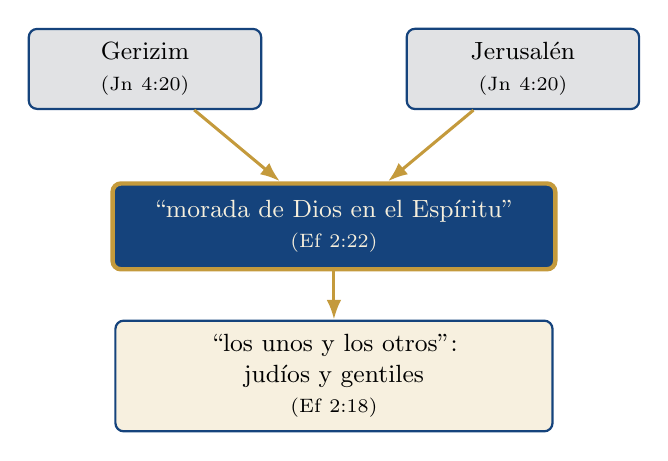
\begin{tikzpicture}[font=\small]
 \node[caja,text width=2.6cm,align=center,fill=gris!18,font=\small] (g) at (-2.4,2.0) {Gerizim\\ {\scriptsize(Jn 4:20)}};
 \node[caja,text width=2.6cm,align=center,fill=gris!18,font=\small] (j) at (2.4,2.0) {Jerusalén\\ {\scriptsize(Jn 4:20)}};
 \node[draw=dorado,line width=1.6pt,fill=azul,text=papiro,rounded corners=3pt,text width=5.2cm,align=center,inner sep=6pt] (t) at (0,0) {``morada de Dios en el Espíritu''\\ {\scriptsize(Ef 2:22)}};
 \node[caja,text width=5.2cm,align=center,font=\small] (p) at (0,-1.9) {``los unos y los otros'': judíos y gentiles\\ {\scriptsize(Ef 2:18)}};
 \draw[-{Latex[length=2.5mm]},dorado,line width=1.1pt](g)--(t); \draw[-{Latex[length=2.5mm]},dorado,line width=1.1pt](j)--(t); \draw[-{Latex[length=2.5mm]},dorado,line width=1.1pt](t)--(p);
\end{tikzpicture}
\end{frame}

\begin{frame}{``En espíritu servimos a Dios''}
\begin{columns}[t,onlytextwidth]
\begin{column}{0.50\textwidth}
\begin{cita}Porque nosotros somos la circuncisión, los que en espíritu servimos a Dios y nos gloriamos en Cristo Jesús, no teniendo confianza en la carne.\fuente{(Flp 3:3, RVR1960)}\end{cita}
\begin{cita}Así que, hermanos, os ruego por las misericordias de Dios, que presentéis vuestros cuerpos en sacrificio vivo, santo, agradable a Dios, que es vuestro culto racional.\fuente{(Ro 12:1, RVR1960)}\end{cita}
\end{column}
\begin{column}{0.48\textwidth}\small
\begin{itemize}
\item \grc{λατρεύοντες} (Flp 3:3) y \grc{λατρεία} (Ro 12:1): el vocabulario del \destacar{culto} del templo.
\item ``Espíritu'' frente a ``carne'' (Flp 3:3), como en Is 31:3.
\item El culto nuevo no suprime el cuerpo: lo ofrece entero. ``Culto racional'' (\grc{λογικὴν λατρείαν}) es el de Jn 4:24 vivido en lo cotidiano.
\end{itemize}
\precision{(textual) NA28 y el texto bizantino leen \grc{πνεύματι θεοῦ λατρεύοντες}, ``los que servimos por el Espíritu de Dios''; la RVR1960 sigue la lectura ``servimos a Dios''.}
\end{column}
\end{columns}
\end{frame}

\begin{frame}{``¡Abba, Padre!''}
\begin{columns}[t,onlytextwidth]
\begin{column}{0.50\textwidth}
\begin{cita}Pues no habéis recibido el espíritu de esclavitud para estar otra vez en temor, sino que habéis recibido el espíritu de adopción, por el cual clamamos: ¡Abba, Padre! El Espíritu mismo da testimonio a nuestro espíritu, de que somos hijos de Dios.\fuente{(Ro 8:15--16, RVR1960)}\end{cita}
\end{column}
\begin{column}{0.48\textwidth}\small
\begin{itemize}
\item Jesús habló de adorar ``al \destacar{Padre}'' (Jn 4:21, 23); Pablo muestra cómo: el Espíritu nos hace decir ``Abba''.
\item \grc{αὐτὸ τὸ πνεῦμα συμμαρτυρεῖ τῷ πνεύματι ἡμῶν}: el Espíritu de Dios testifica \destacar{con} nuestro espíritu. Espíritu con espíritu: la comunión que Jn 4:24 pide.
\item ``Si el Espíritu\ldots{} mora en vosotros\ldots{} vivificará también vuestros cuerpos mortales'' (Ro 8:11).
\end{itemize}
\end{column}
\end{columns}
\end{frame}

\begin{frame}{El postrer Adán, espíritu vivificante}
\begin{columns}[c,onlytextwidth]
\begin{column}{0.50\textwidth}
\begin{cita}Así también está escrito: Fue hecho el primer hombre Adán alma viviente; el postrer Adán, espíritu vivificante.\fuente{(1 Co 15:45, RVR1960)}\end{cita}
\scriptsize\renewcommand{\arraystretch}{1.12}
\begin{tabular}{@{}>{\RaggedRight\arraybackslash}p{1.7cm}>{\RaggedRight\arraybackslash}p{4.0cm}@{}}
\toprule
Gn 2:7 LXX & \grc{ἐγένετο ὁ ἄνθρωπος εἰς ψυχὴν ζῶσαν} \\
1 Co 15:45 & \grc{ὁ ἔσχατος Ἀδὰμ εἰς πνεῦμα ζῳοποιοῦν} \\
\bottomrule
\end{tabular}
\end{column}
\begin{column}{0.48\textwidth}\small
\begin{itemize}
\item El primer Adán \destacar{recibió} aliento (Gn 2:7); el último Adán \destacar{da} vida.
\item Cristo resucitado hace lo que solo el Dios que es Espíritu hace: vivificar (Ez 37:14; Jn 6:63).
\item El cuerpo de resurrección será ``espiritual'' (\grc{πνευματικόν}, 15:44): no inmaterial, sino animado por el Espíritu.
\end{itemize}
\end{column}
\end{columns}
\end{frame}

\begin{frame}{Dios es Espíritu, revelado en Cristo}
\centering
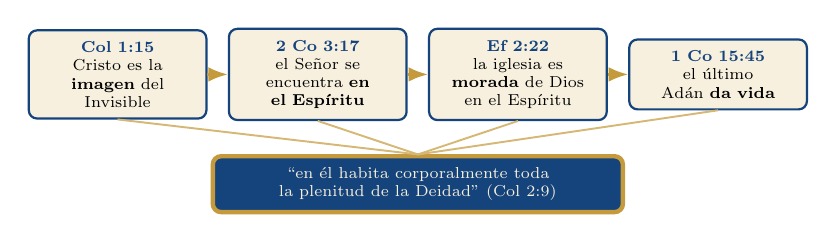
\begin{tikzpicture}[font=\scriptsize,scale=0.82,transform shape]
 \foreach \x/\y/\n/\t/\d in {0/0/a/{Col 1:15}/{Cristo es la \textbf{imagen} del Invisible},
   3.1/0/b/{2 Co 3:17}/{el Señor se encuentra \textbf{en el Espíritu}},
   6.2/0/c/{Ef 2:22}/{la iglesia es \textbf{morada} de Dios en el Espíritu},
   9.3/0/d/{1 Co 15:45}/{el último Adán \textbf{da vida}}}{
  \node[caja,text width=2.4cm,align=center] (\n) at (\x,\y) {\textbf{\textcolor{azul}{\t}}\\ \d};}
 \draw[-{Latex[length=2.5mm]},dorado,line width=1.1pt](a)--(b); \draw[-{Latex[length=2.5mm]},dorado,line width=1.1pt](b)--(c); \draw[-{Latex[length=2.5mm]},dorado,line width=1.1pt](c)--(d);
 \node[draw=dorado,line width=1.6pt,fill=azul,text=papiro,rounded corners=3pt,text width=6.0cm,align=center,inner sep=5pt] (e) at (4.65,-1.7) {``en él habita corporalmente toda la plenitud de la Deidad'' (Col 2:9)};
 \foreach \i in {a,b,c,d}\draw[dorado!70,line width=0.7pt](\i.south)--(e.north);
\end{tikzpicture}\par\medskip
\small\RaggedRight Pablo, judío formado en Dt 4 y en Is 31, no hace imágenes de Dios: mira ``la gloria de Dios en la faz de Jesucristo'' (2 Co 4:6). El Dios que es Espíritu se da a conocer en el Hijo y se da a sí mismo en el Espíritu.
\end{frame}

% ------------------------------------------------------------------
\section{Vivirlo}

\begin{frame}{Adorar sin monte}
\begin{columns}[t,onlytextwidth]
\begin{column}{0.50\textwidth}
\begin{cita}\SENOR{} dijo así: El cielo es mi trono, y la tierra estrado de mis pies; ¿dónde está la casa que me habréis de edificar, y dónde el lugar de mi reposo?\ldots{} pero miraré a aquel que es pobre y humilde de espíritu, y que tiembla a mi palabra.\fuente{(Is 66:1--2, RVR1960)}\end{cita}
\end{column}
\begin{column}{0.48\textwidth}\small
\begin{itemize}
\item Los lugares sirven, pero no contienen a Dios. El \SENOR{} mira al ``humilde de espíritu'' (\heb{נְכֵה־רוּחַ}).
\item Ningún edificio, ritual o emoción garantiza la adoración; tampoco la impiden.
\item ``Cuando ores, entra en tu aposento\ldots{} y tu Padre que ve en lo secreto te recompensará'' (Mt 6:6).
\end{itemize}
\end{column}
\end{columns}
\end{frame}

\begin{frame}{Sin imágenes, ni de piedra ni de la mente}
\begin{columns}[t,onlytextwidth]
\begin{column}{0.50\textwidth}
\begin{cita}¿A qué, pues, haréis semejante a Dios, o qué imagen le compondréis?\fuente{(Is 40:18, RVR1960)}\end{cita}
\begin{cita}Hijitos, guardaos de los ídolos. Amén.\fuente{(1 Jn 5:21, RVR1960)}\end{cita}
\end{column}
\begin{column}{0.48\textwidth}\small
\begin{itemize}
\item \heb{וּמַה־דְּמוּת תַּעַרְכוּ לוֹ}: ``¿qué semejanza le pondréis?''.
\item Hoy pocos tallan ídolos, pero muchos se forman un dios a su medida: un Dios solo ``útil'', solo ``cercano'' o solo ``lejano''.
\item Conocemos a Dios por lo que \destacar{dice} de sí mismo (Dt 4:12) y por el Hijo (Jn 1:18), no por lo que imaginamos.
\end{itemize}
\end{column}
\end{columns}
\end{frame}

\begin{frame}{Cuatro respuestas al Dios que es Espíritu}
\centering
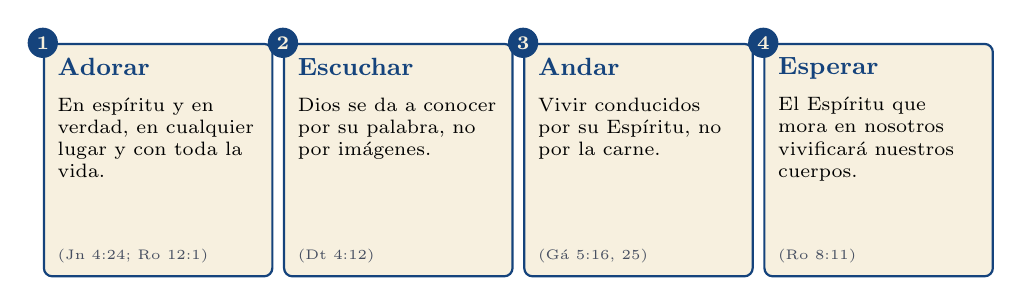
\begin{tikzpicture}
 \foreach \x/\n/\t/\d/\r in {0/1/{Adorar}/{En espíritu y en verdad, en cualquier lugar y con toda la vida.}/{Jn 4:24; Ro 12:1},
   3.05/2/{Escuchar}/{Dios se da a conocer por su palabra, no por imágenes.}/{Dt 4:12},
   6.1/3/{Andar}/{Vivir conducidos por su Espíritu, no por la carne.}/{Gá 5:16, 25},
   9.15/4/{Esperar}/{El Espíritu que mora en nosotros vivificará nuestros cuerpos.}/{Ro 8:11}}{
  \node[caja,anchor=north] (b\n) at (\x,0) {\parbox[t][2.6cm][t]{2.55cm}{\RaggedRight
    {\small\textbf{\textcolor{azul}{\t}}}\\[5pt]\scriptsize \d\par\vfill{\tiny\color{gris}(\r)}}};
  \node[circle,fill=azul,text=papiro,font=\scriptsize\bfseries,inner sep=1.6pt] at (b\n.north west) {\n};}
\end{tikzpicture}\par\medskip
\small\RaggedRight ``Si vivimos por el Espíritu, andemos también por el Espíritu'' (Gá 5:25).
\end{frame}

% ------------------------------------------------------------------
\section{Síntesis}

\begin{frame}{Síntesis}
\begin{tcolorbox}[colback=papiro,colframe=azul,boxrule=1pt,arc=3pt]
\footnotesize ``Dios es Espíritu'' (Jn 4:24). La palabra hebrea \emph{rúaj} une viento, aliento y espíritu: lo invisible que es real y da vida. Dios es el ``Dios de los espíritus de toda carne'' (Nm 16:22): sin cuerpo, sin figura, presente en todo lugar y fuente de toda vida. En Horeb se reveló como \destacar{voz sin figura} (Dt 4:12), y por eso Israel no debía hacer imágenes. En Sicar, Jesús dejó atrás la disputa de los montes: el Padre busca adoradores en espíritu y en verdad. Pablo lo ve cumplido: Cristo es ``la imagen del Dios invisible'' (Col 1:15), en él habita la plenitud ``corporalmente'' (Col 2:9), y la iglesia es ``morada de Dios en el Espíritu'' (Ef 2:22).
\end{tcolorbox}
\scriptsize\renewcommand{\arraystretch}{1.15}
\begin{tabular}{@{}>{\RaggedRight\arraybackslash}p{2.4cm}>{\RaggedRight\arraybackslash}p{9.4cm}@{}}
\toprule
\textbf{Mirada} & \textbf{Aporte} \\ \midrule
Hebrea & \emph{rúaj} (viento, aliento, espíritu); carne y no espíritu (Is 31:3); voz sin figura (Dt 4:12); Dios de los espíritus (Nm 16:22). \\
Judía & el alma y el Santo (Berajot 10a); ``no es cuerpo'' (Maimónides, \emph{Yigdal}); los targumes: ``la gloria'', ``la voz''. \\
Pink & no ``un espíritu'' entre otros; incorpóreo y por eso omnipresente; conocido solo espiritualmente. \\
Paulina & imagen del Invisible; ``el Señor es el Espíritu''; templo en el Espíritu; culto racional; el último Adán da vida. \\
\bottomrule
\end{tabular}
\end{frame}

\begin{frame}{Para la reflexión}
\begin{cita}Mas alábese en esto el que se hubiere de alabar: en entenderme y conocerme, que yo soy \SENOR, que hago misericordia, juicio y justicia en la tierra; porque estas cosas quiero, dice \SENOR.\fuente{(Jer 9:24 [9:23], RVR1960)}\end{cita}
\begin{center}\heb{כִּי אֲנִי יְהוָה עֹשֶׂה חֶסֶד מִשְׁפָּט וּצְדָקָה בָּאָרֶץ}\end{center}
\small
\begin{itemize}
\item ¿Dónde está hoy mi ``monte'': el lugar, el estilo o la emoción sin los que creo que no puedo adorar?
\item ¿Qué imagen de Dios me he formado que no viene de su palabra?
\item ¿Mi culto se queda en la reunión, o llega a mi cuerpo y a mi semana (Ro 12:1)?
\item ¿Vivo como quien tiene en sí el Espíritu del Dios vivo (Ro 8:11)?
\end{itemize}
\end{frame}

% ------------------------------------------------------------------
\section{Glosario}

\begin{frame}{Glosario}
\scriptsize
\begin{columns}[t,onlytextwidth]
\begin{column}{0.49\textwidth}
\begin{description}\setlength{\itemsep}{1pt}
\item[\emph{Aóratos}] (\grc{ἀόρατος}) invisible (Col 1:15; 1 Ti 1:17; He 11:27).
\item[\emph{Basar}] (\heb{בָּשָׂר}) carne; lo perecedero frente al espíritu (Is 31:3).
\item[\emph{Eikón}] (\grc{εἰκών}) imagen (Ro 1:23; 2 Co 4:4; Col 1:15).
\item[\emph{Elohé harujot}] (\heb{אֱלֹהֵי הָרוּחֹת}) ``Dios de los espíritus'' (Nm 16:22; 27:16).
\item[\emph{Gerizim}] (\heb{גְּרִזִים}) monte de la bendición (Dt 11:29); centro del culto samaritano.
\item[\emph{Latreía}] (\grc{λατρεία}) culto, servicio sagrado (Ro 12:1; Flp 3:3).
\item[\emph{Neshamá}] (\heb{נְשָׁמָה}) aliento vital (Gn 2:7; Pr 20:27).
\end{description}
\end{column}
\begin{column}{0.49\textwidth}
\begin{description}\setlength{\itemsep}{1pt}
\item[\emph{Pneûma}] (\grc{πνεῦμα}) viento, aliento, espíritu (Jn 3:8; 4:24).
\item[\emph{Pneumatikós}] (\grc{πνευματικός}) espiritual (1 Co 2:15; 15:44).
\item[\emph{Proskynéō}] (\grc{προσκυνέω}) adorar, postrarse (Jn 4:20--24).
\item[\emph{Rúaj}] (\heb{רוּחַ}) viento, aliento, espíritu (Gn 1:2; Ez 37:9).
\item[\emph{Sōmatikôs}] (\grc{σωματικῶς}) corporalmente (Col 2:9).
\item[\emph{Temuná}] (\heb{תְּמוּנָה}) figura, forma visible (Dt 4:12, 15).
\item[\emph{Tsélem}] (\heb{צֶלֶם}) imagen (Gn 1:27).
\end{description}
\end{column}
\end{columns}
\end{frame}

% ------------------------------------------------------------------
\section{Referencias}

\begin{frame}{Referencias}
\fontsize{5.4}{6.4}\selectfont
\begin{columns}[t,onlytextwidth]
\begin{column}{0.49\textwidth}
\refapa{Chávez, M. (1992). \emph{Diccionario de hebreo bíblico}. Editorial Mundo Hispano.}
\refapa{Dunn, J.~D.~G. (1998). \emph{The theology of Paul the apostle}. Eerdmans.}
\refapa{Elliger, K., \& Rudolph, W. (Eds.). (1997). \emph{Biblia Hebraica Stuttgartensia} (5.ª ed.). Deutsche Bibelgesellschaft.}
\refapa{García Martínez, F. (1992). \emph{Textos de Qumrán}. Trotta.}
\refapa{Gerizim, Mount. (2007). En F. Skolnik \& M. Berenbaum (Eds.), \emph{Encyclopaedia Judaica} (2.ª ed.). Macmillan Reference USA.}
\refapa{Hays, R.~B. (1989). \emph{Echoes of Scripture in the letters of Paul}. Yale University Press.}
\refapa{MacArthur, J. (2011). \emph{Biblia de estudio MacArthur} (notas). Grupo Nelson.}
\refapa{Maimónides. (s.f.). \emph{Comentario a la Misná} [Sanedrín 10:1]; \emph{Mishné Torá} [Yesodé haTorá 1:7--9; Teshuvá 3:7]. Sefaria. https://www.sefaria.org}
\refapa{Maimónides. (s.f.). \emph{Guía de los perplejos} [I:40] (S. ibn Tibbon, Trad. hebrea). Sefaria. https://www.sefaria.org}
\refapa{Nestle, E., \& Aland, K. (Eds.). (2012). \emph{Novum Testamentum Graece} (28.ª ed.). Deutsche Bibelgesellschaft.}
\end{column}
\begin{column}{0.49\textwidth}
\refapa{Pink, A.~W. (2020). \emph{Los atributos de Dios} (E. Rodríguez Cruz, Trad.). Chapel Library. (Obra original publicada en 1930)}
\refapa{Rahlfs, A., \& Hanhart, R. (Eds.). (2006). \emph{Septuaginta} (Ed. rev.). Deutsche Bibelgesellschaft.}
\refapa{Rashi. (s.f.). \emph{Comentario a la Torá} [Gn 1:2; Nm 16:22; 27:16]. Sefaria. https://www.sefaria.org}
\refapa{\emph{Santa Biblia: Reina-Valera 1960}. (1960). Sociedades Bíblicas en América Latina.}
\refapa{\emph{Sidur} [\emph{Yigdal}]. (1981). \emph{The Metsudah siddur}. Sefaria. https://www.sefaria.org}
\refapa{Steinsaltz, A. (Ed.). (2017). \emph{Koren Talmud Bavli: Edición William Davidson} [Berajot 10a]. Sefaria. https://www.sefaria.org}
\refapa{Strong, J. (1890). \emph{The exhaustive concordance of the Bible}. Hunt \& Eaton.}
\refapa{\emph{Targum Ónkelos} [Gn 1:2; Éx 24:10; Nm 16:22; Dt 4:12]; \emph{Targum Jonatán a los Profetas} [Is 31:3]. (s.f.). Sefaria. https://www.sefaria.org}
\refapa{Tov, E. (2012). \emph{Textual criticism of the Hebrew Bible} (3.ª ed.). Fortress Press.}
\refapa{Vermes, G. (2004). \emph{The complete Dead Sea Scrolls in English} (Ed. rev.). Penguin.}
\refapa{Vine, W.~E. (1999). \emph{Diccionario expositivo de palabras del Antiguo y del Nuevo Testamento exhaustivo}. Caribe.}
\end{column}
\end{columns}
\par\smallskip{\color{gris}Las citas bíblicas son de la Reina-Valera 1960; ``Jehová'' se reemplaza por \SENOR. Hebreo: BHS; griego: NA28 y LXX de Rahlfs-Hanhart. Fuentes judías: Sefaria; lo rabínico se marca como \emph{precisión}.}
\end{frame}

\end{document}
